\documentclass[11pt]{article}
\usepackage[utf8]{inputenc} %UTF8 stöd så att jag kan skriva åäö
\usepackage[swedish]{babel}
\usepackage{hyperref}
\usepackage{graphicx}
\usepackage{fixltx2e}
\usepackage{float}
\usepackage[style=authoryear, backend=biber, natbib=true]{biblatex}

\addbibresource{referenser.bib}


\begin{document}

\title{NFC Lås}

\date{2012-05-20}

\author{Fredrik Einarsson\\
    	Robin Gabre\\
		Jonas Hemlin\\
		Sebastian Karlsson\\
		Daniel Moreau\\ 
		Kristofer Tapper\\}

\maketitle
\newpage

\section*{Förord}
Denna rapport ingår i ett kandidatarbete utfört vid Institutionen för Data- och informationsteknik, Chalmers tekniska högskola under våren 2013. Rapporten beskriver utvecklingen av ett NFC-baserat låssystem bestående av en Android-applikation samt mjukvara till en mikrokontroller av Arduino-typ.

Projektgruppen önskar tacka Lars Svensson för den tid han har lagt ner för att leda projektet i rätt riktning.

\newpage

\renewcommand{\abstractname}{Abstract}
\begin{abstract}
In english motherfucker.
\end{abstract}
\newpage

\renewcommand{\abstractname}{Sammanfattning}
\begin{abstract}
Mobiltelefonen utökas idag ständigt till att klara av att utföra fler och fler uppgifter åt dess användare. De saker, vars funktioner nu erbjuds genom dagens mobiltelefoner, behöver användaren alltså inte längre bära med sig. Det här arbetet syftar till att ersätta nyckelknippan genom att ge mobiltelefonen funktionen att låsa upp en dörr. Därav redogör rapporten för hur en prototyp av ett låssystem designas och implementeras, och detta är också rapportens syfte.

För att kunna erbjuda den önskade funktionaliteten har en låsenhet utvecklats kring Arduino-plattformen vilken har möjligheten att styra en elektrisk låskolv. Vidare har en mobilapplikation för Android utvecklats, vilken användaren använder för att kunna låsa eller låsa upp en dörr med en integrerad låsenhet. Mobilapplikationen kommunicerar med låsenheten via NFC(Near Field Communication).

Säkerheten i systemet består i att användaren verifierar sig mot mobilapplikationen med förvald PIN-kod och kommunikationen är krypterad med krypteringsalgoritmen RSA\footnote{Efter upphovsmännen Ron Rivest, Adi Shamir och Len Adleman} med 512 bitars nycklar.

%Slutsatser
\end{abstract}
\newpage

\section*{Ordlista/Terminologi}
\begin{description}
\item[Aktivitet] En Java-klass som representerar en enstaka fokuserad uppgift. Ses vanligen som en skärm i Android.
\item[Användare] En person som använder mobilapplikationen.
\item[Android] Ett öppet mobilt operativsystem för främst smartphones och pekplattor.
\item[Android beam] En teknologi för att sända data mellan två Androidenheter via NFC.
\item[API] (\textit{Application Programming Interface}) - en regeluppsättning för hur en viss programvara kan kommunicera mot annan programvara.
\item[Bluetooth] Standard för trådlös kommunikation mellan enheter.
\item[Börkrav] Krav som bör ha uppfyllt för en bra produkt
\item[Ciphertext] 
\item[DEP](\textit{Data Exchange Protocol}) - ett transportprotokoll på RF-nivå.
\item[DSAP] Destination service access point, adress som utgör mål för NFC kommunikation.
\item[Key-value-store] Abstrakt datatyp bestående av en samling av par där nyckeln är unik.
\item[Kryptoanalys]
\item[Kryptosystem] 
\item[LLCP](\textit{Logical Link Control Protocol})  Det protokoll som dikterar hur NFC-kommunikation sköts på länknivå.
\item[Låsenhet] Den del utav den utvecklade prototypen vilken är integrerad i låset.
\item[Manifest] Är en fil i ett Androidproject som specificerar globala inställningar för applikationen.
\item[Material] De fysiska delarna vilken prototypen utgörs av.
\item[Mobil plånbok] En ansats till att ersätta plånboken med en applikation i en smart telefon.
\item[NFC] (\textit{Near Field Communication}) - En trådlös kommunikationsteknik över korta avstånd. 
\item[NFC-Forum] En organisation med målet att sprida och utveckla teknologin NFC.
\item[NDEF] (\textit{NFC Data Exchange Format}) Ett dataformat som specificerar hur data skall skickas och vad det är för data som skickas.
\item[OSI-modellen] en konceptuell modell för datorkommunikation i 7 lager.
\item[Plaintext] Klartext, ett okrypterat meddelande, används i krypteringssammanhang
\item[Primärnyckel] Unik kolumn(er) i en databas.
\item[Relationsdatabas] Databas där information är organiserad i relationer.
\item[RF] Radiofrekvens.
\item[RSA] Algoritm som används vid asymmetrisk kryptering.
\item[SDP] (Service Discovery Protocol)  är ett protkoll som används när avsändare inte känner DSAP hos målenhet.
\item[Server] Är ett datorsystem som har till uppgift att serva andra system.
\item[Skallkrav] Krav som skall vara uppfyllda i prototypen.
\item[Smart telefon] En mobil enhet som kan användas både som avancerad mobiltelefon och som handdator.
\item[SNEP] (Simple NDEF exchange protocol) Detta protokoll beskriver utbytet av data vid användning av NFC.
\item[SSAP] (Source service access point)  Den adress som brukande applikation tilldelats vid användandet av NFC.
\item[Target] Målenhet för NFC kommunikation
\item[Verktyg] Källkodsbibliotek, utvecklingmiljöer och specifikationer.
\item[Wifi] Teknik för trådlösa nätverk.
\end{description}
\newpage


\setcounter{secnumdepth}{4}
\setcounter{tocdepth}{4}
\tableofcontents
\newpage


\section{Inledning}
När mobiltelefonen först lanserades var den stor, otymplig och dyr, med kommunikation som enda syfte. Sedan dess har utvecklingen eskalerat kraftigt och allt fler funktioner har integrerats, medan själva mobiltelefonen har gjorts mindre, smidigare och mer tillgänglig för allmänheten. Idag äger i princip alla svenskar en mobiltelefon och byter dessutom dessa ofta, då det är både relativt billigt att köpa en ny samt att tekniken snabbt framskrider. I och med den stora efterfrågan på mobiltelefoner är branschen hårdare än någonsin för producenterna och för att deras produkter ska bli konkurrenskraftiga på den ständigt utvecklande marknaden måste produkterna oupphörligt innehålla nya och smartare funktioner.

På senare tid har övergången till så kallade smarta telefoner ytterligare bidragit till att öka funktionaliteten hos mobiltelefonen. Numera är den inte enbart ett redskap för kommunikation, utan en enhet med lika många eller till och med fler funktioner än en persondator. En av anledningarna till denna utveckling är framstegen inom integrerade kretsar och dess tillverkningsteknik. Dessa faktorer har bidragit till att fler transistorer kan placeras på en mindre yta (Intel Corporation, 2005) och därmed göra elektronikkomponenter både mindre, strömsnålare, snabbare och mer funktionella. Den direkta följden av detta är att mobiltelefonen nu kan inrymma både funktionaliteten av fler kringenheter, samt inneha kraft nog att hantera dem alla.\\
Wifi och Bluetooth är exempel på tekniker för kommunikation vilka i stort sett alltid finns inbyggt i en mobiltelefon och nu, vilket Deffree (2012) skriver, börjar även en ny kommunikationsteknik få allt större utbredning, NFC (Near Field Communication). Detta är en teknik för tillförlitlig kommunikation över korta avstånd, vilken bland annat ligger till grund för en senare ansats att försöka ersätta något vi alltid bär med oss, plånboken. Tanken med denna produkt som i många fall kallas den mobila plånboken, vilken Timalsina (2012) beskriver, är att göra anspråk på att ersätta våra kontanter, rabatt- och kreditkort med programvara i mobiltelefonen.\\
Idén bakom detta arbete baseras på samma tankegångar vilka ligger bakom utvecklingen av den mobila plånboken; att ersätta något vi alltid bär med oss. Kandidatarbetet åsyftar till att ersätta nyckeln genom att utveckla en prototyp av ett låssystem som tillåter användaren att på ett snabbt och bekvämt sätt låsa upp dörren till sitt hem med sin mobiltelefon. För att möjliggöra denna funktionalitet används samma kommunikationsteknik som ligger till grund för den mobila plånboken, NFC.\\
Resultatet av kandidatarbetet kan vara en mycket åtråvärd produkt för privatpersoner vilka är trötta på att leta efter sina hemnycklar samt önskar en flexiblare lösning än den klassiska nyckeln. Målet är att ytterligare följa trenden mot en allt mer funktionell mobiltelefon genom att också använda den som en nyckel.\\
Visionen för en färdig produkt av detta slag, och alltså inte för resultatet av detta kandidatarbete, är att produkten ska kunna användas i större företag där det finns hundratals dörrar som utrustats med den utvecklade låsenheten samt tusentals anställda som alla använder sin mobiltelefon för att kontrollera låsenheterna. Många accessnivåer kan finnas där en specifik användare kan ingå i valfritt antal. Produkten kan underhållas av en central enhet som snabbt, smidigt och säkert kan konfigurera om systemet efter givna instruktioner.\\
Det finns också andra visioner för en färdig produkt av detta slag. Låssystemet behöver nödvändigtvis inte vara ett stort, relativt komplext och centraladministrerat system utan kan istället vara litet, simpelt och mobilt system vilket kan användas i cykellås eller hänglås.
\subsection{Syfte}
Syftet med rapporten är att redogöra för hur en prototyp av ett låssystem designas och implementeras. Låssystemet består av en mobilapplikation och en mikrokontroller där mikrokontrollern är integrerad i låset samt exekverar egenutvecklad mjukvara. Skulle det visa sig att produkten inte uppfyller kravspecifikationen(se bilaga HAJ) ska en analys genomföras i vilken en fullständig slutprodukt beskrivs teoretiskt.

\subsection{Utmaningar}
Under planeringsfasen av låssystemet identifierades tre huvudsakliga utmaningar vilka beskrivs punktvis nedan.

\begin{itemize}

\item Stora delar av NFC:s kommunikationsstack måste implementeras för mikrokontrollern och den måste utformas efter hur Androids NFC-stack är uppbyggd. Att implementera denna kommunikationsstack medför en större utmaning då den är relativt komplex, innehåller ett flertal olika nivåer, och dokumentation kring Androids implementation är bristfällig. någon källa här kanske??

\item Att implementera en Android-applikation vilken ska innehålla funktioner för att kommunicera mot mikrokontrollern via NFC. Androidutveckling medför ytterligare svårigheter jämfört med vanlig mjukvaruutveckling då hänsyn måste tas till Androids egenheter, vilka beskrivs närmare i teoriavsnitt 3.2. En förståelse för de källkodsbibliotek vilka styr NFC-kommunikationen måste också byggas upp. 

\item Att implementera säkerhet vid NFC-kommunikation mellan två enheter vilka använder olika programmeringsspråk. Då en mikrokontroller generellt inte har mycket minne eller hög klockfrekvens kan dessa egenskaper skapa utmaningar då säkerhet i form av kryptering ofta kräver omfattande beräkningskapacitet, vilket beskrivs närmare i teoriavsnitt 3.1.2.4. Den utmaningen vilken uppkommer då olika programmeringsspråk används är problem med varierande datarepresentationer och implementationer av funktioner, metoder och klasser.

\end{itemize}

\subsection{Omfattning}
Rapporten beskriver endast processen för utvecklingen av en prototyp utav ett låssystem vilket beskrivs i avsnitt 4. Vidare beskriver rapporten de nödvändiga förkunskaperna vilka krävs för utvecklingen av en sådan prototyp. Prototypen skall kortfattat nyttja kommunikation via NFC med applicerad säkerhet och därför är förkunskaper inom dessa ämnen nödvändiga.\\
Mobilapplikationen begränsas till endast Android eftersom det är lättillgängligt, välkänt och lämpligt för användningsområdet. Denna avgränsning kommer också naturligt av att det bara finns stöd för NFC hos ett fåtal telefoner där merparten av dem är baserade på Android.\\
Låsenheten baseras på en mikrokontroller ur Arduino-plattformen då plattformen är användarvänlig (McRoberts, 2010) , har en relativt låg prisbild samt att flertalet källkodsbibliotek finns vilka kan underlätta implementeringen av låsenheten. Vidare har Arduino-plattformen stöd för NFC i form av ett färdigutvecklat påstickskort, en så kallad sköld(fotnot 1), med tillhörande källkodsbibliotek.\\
Fokus ligger på att utveckla en prototyp innehållande en låsenhet samt tillhörande mobilapplikation för privatpersoner, alltså inte för ett större företag. Då flera låsenheter eller flera användare av mobilapplikationen läggs till ökar komplexiteten för hela projektet och andra krav kommer att ställas på lösningen.\\
(fotnot 1) från engelskans shield

\section{Metod}
I den initiala fasen genomförs en analys från användarens perspektiv där de krav användaren kan ställa på prototypen listas. Dessa krav utformas sedan från låssystemets perspektiv och sammanställs till en kravspecifikation. Utifrån kravspecifikationen väljs de material, det vill säga de fysiska delarna vilken prototypen utgörs av, vilka är mest lämpade för utformningen av prototypen.\\
Under designfasen av projektet väljs hur prototypens funktionalitet distribueras ut i låssystemet och ett kommunikationsprotokoll för systemets delar sammanställs. All funktionalitet som låssystemet innehåller delas upp på prototypens två enheter. Kommunikationsprotokollet beskriver hur datan som skickas mellan enheterna är uppbyggd, hur kommunikationsförloppet mellan enheterna ser ut samt hur säkerhet appliceras till kommunikationen.\\
Projektet övergår nu till en iterativ arbetsgång där ytterligare funktionalitet, utifrån kravspecifikationen, försöker implementeras för varje iteration. För att kunna utföra en iteration undersöks vilka eller vilket verktyg såsom källkodsbibliotek, utvecklingsmiljöer och information som krävs för att implementera funktionaliteten. Verktygen utvärderas och de som bedöms kunna bidra till, eller underlätta för implementation av den sökta funktionaliteten, väljs ut. Verktygen används sedan för fortskridandet av iterationen. Den tillagda funktionaliteten utvärderas och om den lever upp till kravspecifikationen påbörjas nästa iteration, men skulle den nyligen tillagda funktionalitet inte uppfylla de krav som ställs undersöks vad som är möjligt att ta med utav den nyligen tillagda funktionaliteten till nästa iteration eller om resultatet av iterationen måste kasseras.
\section{Teori}
I detta kapitel beskrivs den teori som är nödvändig att förstå vid konstruktionen av prototypen. Teorin bidrar till en ökad förståelse men bidrar framförallt till det direkta framskridandet av projektet.\\
Eftersom prototypen använder NFC-teknik som kommunikationsmetod är kunskaper inom NFC relevant. Kunskaper inom NFC, och inte bara inom dess användande, är främst nödvändig för utvecklingen av mjukvaran till mikrokontrollern då kommunikationsstacken behöver implementeras från grunden. Detta står i kontrast till utvecklandet av Android-applikationen där kunskaper om användandet av Androids API för NFC är nödvändiga och kunskaper inom dess implementation är mindre viktiga.\\
Vidare är kunskaper inom säker kommunikation relevant eftersom NFC inte har någon inbyggt säkerhet. En applikation som nyttjar NFC bör därför själv implementera säkerhet om behov finns och eftersom ett låssystem skall konstrueras är säkerhet ett krav. Säker kommunikation kan uppnås på många olika sätt och därför är kunskap för att både välja rätt metod och kunskap om den valda metodens implementation av stor vikt.\\
Utvecklingen av Android-applikationen kräver förutom kunskap i Java-programmering även kunskap kring applikationsutveckling för Android vilket tas upp i detta kapitel. Bland annat har applikationer för Android en speciell livscykel som är nödvändig att känna till. Det är även nödvändigt att känna till de Android-specifika API:er som finns att tillgå. Särskilt bör vetskap om de Android-specifika API:er för kommunikation via NFC besittas.\\
För att utveckla en applikation till Arduino-plattformen krävs förutom kunskaper inom C++-programmering även kunskap om Arduino vilket behandlas i detta kapitel. En Arduino har inte något operativsystem vilket gör att en Arduino-applikation kör direkt på den underliggande hårdvaran. Det betyder att kunskaper kring hur kretskorten ser ut måste beskrivas. Vidare behöver kännedom om hur kretskorten kommunicerar med varandra redogöras. Slutligen bör kunskaper angående de nödvändiga Arduino-specifika källkodsbibliotek samt hur Arduino kommunicerar via NFC beskrivas.
\subsection{NFC}
NFC (Near Field Communication) är en trådlös kommunikationsteknik över avstånd upp till ungefär 10 cm och tekniken standardiserades år 2006 (Timalsina 2012). Vidare skriver Timalsina (2012) att NFC baseras på RFID (Radio Frequency Identification), vilket är en väletablerad trådlös kommunikationsteknik som funnits sedan 1983, och bygger vidare på RFID genom att erbjuda tvåvägskommunikation mellan två enheter med inbyggt stöd för NFC.\\ 
Tekniken bygger på att två mikrochips med stöd för NFC-teknik kommunicerar med varandra genom magnetisk induktion och Timalsina (2012) beskriver att kommunikationen mer specifikt baseras på att ett mikrochips modifierar det andra mikrochipsets magnetfält genom att generera radiovågor med frekvensen 13.56 Mhz. Denna modifiering ger upphov till att data kan skickas i hastigheter från 106 Kbps upp till 424 Kbps. Dock kan endast en enhet i taget modifiera den andra enhetens magnetfält vilket ger att kommunikationen endast är halv-duplex, det vill säga att kommunikation endast kan ske i en riktning i taget.\\
Kommunicerande enheter kan vara antingen passiva eller aktiva. Aktiva enheter har strömförsörjning och återfinns till exempel i mobiltelefoner medan passiva enheter saknar strömförsörjning och återfinns till exempel som taggar på posters eller i busskort (Timalsina 2012). Två aktiva enheter kan kommunicera mot varandra. Aktiva enheter kan även kommunicera mot passiva enheter genom att den aktiva enheten ger strömförsörjning till den passiva enheten med hjälp av magnetisk induktion. Två passiva enheter kan inte kommunicera eftersom inget magnetfält uppstår utan tillförd energi (Timalsina 2012).\\
NFC Forum(2013) standardiserade NFC-tekniken år 2006 och är den organisation vilken har ansvar för att ta fram de specifikationer som gör kommunikation via NFC möjlig mellan olika typer av enheter. De har också ansvar för att sprida och uppmuntra användandet av NFC-teknik samt utbilda företag med målet att företagen ska följa de officiella specifikationerna så att tekniken kan fungera sömlöst mellan enheter från olika tillverkare.\\
I de följande teoriavsnitten beskrivs de protokoll vilka NFC Forum har specificerat för att möjliggöra kommunikation mellan två aktiva enheter. Dessa protokoll utgör den NFC-stack vilken båda enheterna i kommunikationen måste implementera. Vidare täcker protokollen hela OSI modellen förutom applikationslagret med tillhörande säkerhet då detta inte ingår i NFC-stacken.

\subsubsection{NFC Stack}
NFC-stacken är uppbyggd av ett antal protokoll vilka sträcker sig i stort sett över hela OSI-modellen, då endast applikationslagret med tillhörande säkerhet ej ingår i NFC-stacken. Listan nedan är en kort översikt över de protokoll vilka ingår i NFC-stacken och NFC-stackens motsvarande OSI-lager gås igenom uppifrån och ned.

\begin{itemize}
\item Data som sänds mellan två aktiva NFC-enheter kappslas in i ett meddelande av typen NDEF(\textit{NFC Data Exchange Format}). Informationen ligger som ett eller flera fält i NDEF-meddelandet som så kallade NDEF-\texttt{records}. 

\item Vidare används protokollet NPP(\textit{NDEF Push Protocol}) eller SNEP(\textit{Simple NDEF Exchange Protocol}) för att utbyta NDEF-meddelanden mellan två aktiva NFC-enheter. Då NPP har ersatts av SNEP kommer bara SNEP att beskrivas.

\item För att upprätta och hantera en länk mellan två aktiva NFC-enheter används LLCP(\textit{Logical Link Control Protocol}). Protokollet hanterar också dataöverföringen mellan enheterna och ser till att den görs utan förluster.

\item Den fysiska överföringen av bitarna hanteras av RF-protokollen där bland annat hur och i vilka hastigheter data kan skickas specifieras.

\end{itemize}

%Bild
%Bildtext: Figur 1. Här visas NFC-stackens protokoll i förhållande till vilket lager i OSI-modellen de utgör.

\paragraph{NDEF}

NDEF(\textit{NFC Data Exchange Format}) (NFC Forum, 2006) är utformat för att kapsla in applikationsdatan på ett effektivt sätt med minimal overhead. NDEF-meddelanden byggs upp av ett eller flera records enligt figur 2, där ett \texttt{record} innehåller applikationsdatan från en applikation. NDEF garanterar inte att leverans av data är tillförlitlig och specificerar således inte vad målenheten skall göra vid mottagandet av ett felaktigt utformat NDEF-meddelande. Detta lämnas till brukande applikationer att komplettera med datagarantier och felhantering som gemensamt brukar kallas QOS (\textit{Quality Of Service}).


%Bild
%Bildtext: Figur 2. Ett NDEF meddelande består av en eller flera records.

Varje \texttt{record} utformas efter en fördefinierad struktur, vilken är illustrerad i figur 3, och består av ett antal fält. Det första fältet är en header, som sedan följs av  \texttt{type length} ,  \texttt{payload length} ,  \texttt{ID length} ,  \texttt{type} ,  \texttt{ID}  och till sist  \texttt{ payload} .

%Bild
%Bildtext: Figur 3. Utformningen av ett record.

\begin{itemize}
\item \textbf{Header.} En record header är en byte lång där varje bit har olika betydelser.

\begin{itemize}
\item Den första biten är \texttt{MB}, vilken är en förkortning av message begin och indikerar att detta är den första record i NDEF meddelandet. Denna bit är ettställd i första record, nollställd i övriga.
\item Den andra biten är \texttt{ME}, vilken är en förkortning av message end och indikerar att detta är den sista record i NDEF-meddelandet. Denna bit är endast ettställd i sista record, nollställd i övriga.
\item Den tredje biten är \texttt{CF}, vilken är en förkortning av chunk flag och ettställd indikerar denna att NDEF-meddelandet är chunked. Chunk-mekanismen tillåter att ett stort datapaket delas upp över flertalet records. Denna mekanism kommer inte att behandlas i denna text då den utvecklade mjukvaran inte nyttjar detta.
\item Den fjärde biten är \texttt{SR} vilken är en förkortning av short record och ettställd indikerar att payload length utgörs av en byte istället för fyra. Detta används då en datamängd på mindre än 256 byte skall överföras.
\item Den femte biten är \texttt{IL} vilken nollställd indikerar att \texttt{ID length} fältet inte existerar i record. Om \texttt{IL} är ettställd existerar fältet.
\item De sista bitarna, bit sex till åtta, bildar \texttt{TNF} vilken är en förkortning av type name format och definierar strukturen av type-fältet i record. Flertalet värden på TNF fältet finns, men det värde vilket är relevant för den utvecklade mjukvaran är 0x02 vilket står för Media-type. Media-type inrymmer allt från enkel text till bilder och video.
\end{itemize}

\item \textbf{Type Length.} Definerar hur många bytes som utgör Type-fältet.
\item \textbf{Payload length 0-3.} Varje delfält i payload är en byte stort vilket ger payload length-fältet en total storlek på fyra byte. Payload length definierar storleken på payload fältet vilket huserar applikationsdatan. I en record med SR nollställd kan payload- fältet vara $8*2^8$ byte stort, det vill säga 4,29 gigabyte. Med SR ettställd kvarstår enbart ett payload lenght-fält vilket ger payload-fältet en maximal storlek på 255 byte.
\item \textbf{Type.} Detta fält definierar vilken typ av data payload-fältet innehåller. Värdet på detta fält måste följa de kraven vad gäller struktur och kodning vilket specificerats av TNF-fältet i header. Type-fältet används för att ange vilken applikation meddelandets data tillhör, men om detta inte behöver specifiseras kan typvärdet “text/plain” anges vilket står för att innehållet i payload är ASCII-formaterad text.
\item \textbf{ID.} Värdet på detta fält är unikt och utgör en unik identifierare kallad URI. Records kan således skiljas åt genom att studera värdet av URI, och NDEF garanterar att detta nummer är unikt genom att tillhandahålla en generator.
\item \textbf{Payload.} Detta fält huserar applikationsdata.
\end{itemize}


\paragraph{SNEP} 
SNEP(Simpel NDEF exchange protocol) (NFC Forum, 2011) är det protokoll i NFC-stacken som hanterar utbytet av NDEF-meddelanden. SNEP är ett så kallat request/response protokoll, en klient skickar en SNEP-förfrågan till en server vilken, beroende på förfrågans innehåll, returnerar ett passande svar om det erfordras.

\subparagraph{Förfrågningar}
SNEP specificerar förfrågans utseende enligt figur 4.

%bild
%bildtext: Figur 4. Utformningen av en SNEP-förfråga

\begin{itemize}
\item \textbf{Version.}Detta fält definierar vilken SNEP-version förfrågan bygger på. Versionsfältet är indelat i två delfält kallat Major och Minor om fyra bitar vardera, där Major huserar heltalet av versionsnumret och Minor huserar decimaldelen av versionsnumret. För att genomföra en SNEP-förfråga måste klient och server förstå varandra och deras förmåga att förstå varandra avgörs av SNEP-versionen. Vid mottagande av en SNEP-förfrågan kontrollerar servern versionsnumret. Stämmer numret helt överens med den version som servern använder kan SNEP-sessionen fullbordas. Stämmer Major delen men inte Minor är det möjligt att slutföra sessionen om servern anpassar sig efter klienten, men skiljer sig Major delen kan sessionen inte genomföras och servern ger avslag på den mottagna förfrågningen.
\item \textbf{Request.} Detta fält är åtta bitar stort och anger typen av SNEP-förfråga. Olika SNEP-förfrågningar erfordrar olika svar från servern.
\item \textbf{Length.} Detta fält anger hur många byte som utgör informationsfältet. Length-fältet är fyra byte långt vilket resulterar i att informationsfältet kan innehålla 4,29 gigabyte data.
\item \textbf{Information} Innehållet i detta fält beror på innehållet i Request-fältet, det vill säga vilken sorts förfråga det är. Vanligtvis huseras ett NDEF meddelande i informationsfältet.
\end{itemize}

De förfrågningar en klient kan begära från en server är Continue, Get, Put samt Reject. De två vanligaste förfrågningarna och de vilka är av relevans för projektet är Put och Get vars betydelse och användning förklaras nedan.

\textbf{Put.} En Put-förfråga har kod 0x02 och utformas enligt figur 4. Förfrågan innebär att klienten ber servern att ta emot det inkapslade NDEF meddelandet utan att servern returnerar något förutom ett Success-svarsmeddelande om förfrågningen kunde tas emot. 

%bild
%bildtext: Figur 4. Utformning av en Put-förfråga.


\textbf{Get.} En Get-förfråga har kod 0x01 och utformas enligt figur 5. Förfrågan innebär att klienten ber servern att returnera information inkapslat i ett NDEF-meddelande. Vilken information klienten önskar specificeras i NDEF-meddelandet vilket huseras i Get-förfrågans information-fält. Dock utgör de fyra första byten i information-fältet fältet Acceptable Length vilket anger maxstorleken av serverns returnerande NDEF-meddelande. 

%bild
%bildtext. Figur 5. Utformning av en Get-förfråga.

\subparagraph{Svarsmeddelanden}
SNEP specificerar utformningen av ett svarsmeddelande enligt figur 6. Fälten i ett svarsmeddelande fyller samma funktion som i en förfråga med undantag för andra byten vilket i ett svarsmeddelande kallas Respons istället för en förfrågas Request. Respons innehåller koden för det typ av svarsmeddelande vilket skickas.

%bild
%bildtext: Figur 6. Utformning av ett SNEP-svarsmeddelande.


SNEP-svarsmeddelanden följer sällan den specifiserade utformningen. Det är enbart svar på Get-förfrågningar som fullt ut följer det generella utseendet hos ett svar. Vanligt förekommande svar är följande.

\textbf{Response.} Fyller samma funktion som Request-fältet. Dock innehåller denna andra koder som alla är av svarstyp.

SNEP svar följer ganska sällan det fördefinerade utseendet. Det är enbart svar på Get-förfrågningar som fullt ut följer det generella utseendet hos ett svar. Vanligt förekommande svar är följande.

\begin{itemize}
\item \textbf{Success.} Detta svar indikerar att servern klarat av att genomföra klientens Get eller Put förfrågan. Utformningen på Success-svaret skiljer sig beroende på om det ges som svar på en Get eller Put förfrågan. I fallet Get följer svaret den generella utformningen med response satt till 0x81 vilket indikerar success. I information-fältet huseras NDEF-meddelandet som ges som svar på Get-förfrågan. I fallet Put sätts response till 0x81, men informations-fältet närvarar ej.
\item \textbf{Not found.} Detta svar ges om servern inte klarar av att returnera önskat svar till klienten. Svarskoden är 0xC0 och inget information-fält förekommer.
\item \textbf{Bad request.} Ges om förfrågningen inte följer fördefinierat utseende. Svarskoden är 0xC2 och inget information-fält förekommer.
\item \textbf{Not implemented.} Detta svar ges om servern inte stödjer den funktionalitet som klienten ber om i förfrågan. Detta svar lämpar sig väl om felaktig request-kod angivits i förfrågan. Inget information-fält förekommer.
\item \textbf{Unsupported version} Ges då klientens SNEP version inte stämmer överens med vad servern kan hantera. Major-delen av version-fältet skiljer sig åt alternativt klarar servern inte av att överbygga de skillnader som olika Minor-värden medför. Inget information-fält förekommer.
\end{itemize}

Alla NFC-enheter har som krav att ha en SNEP-server process körandes. På så vis garanteras att all SNEP kommunikation behandlas. Denna garanti förenklar för både ovanliggande applikationslager som underliggande LLC-lager.

\paragraph{LLCP}
LLCP(Logical Link Control Protocol) (NFC Forum 2, 2011) är protokollet som sköter samtliga datalänkar med andra NFC enheter. För att öka överskådligheten hos protokollet har det delats upp i fyra centrala delar: Media access mappning, länkhanteraren, förbindelselös transport och förbindelseorienterad transport. NFC-stacken ser med dessa delar ut som figuren nedan visar.

%bild

\subparagraph{Media access mappning}
Knyter samman ovanliggande protokoll med de RF-protokoll (3.1.1.4), vilka styr tekniken som står för den faktiska överföringen av data mellan två NFC enheter. 

\subparagraph{Länkhanteraren}
Detta är en process som styr all NFC-kommunikation och körs på samtliga enheter som stödjer NFC. Länkhanteraren serialiserar all kommunikation till och från NFC-enheter samt kan hantera flera parallella datalänkar och sköta övervakningen av deras aktuella tillstånd.\\
Ytterligare en viktig funktion som länkhanteraren fyller är att genomföra ett så kallat symmetriförfarande. Eftersom NFC är halvt duplex, dvs. kommunikation kan ske i båda riktningar men endast en part i kommunikationen får sända samtidigt, måste länkhanteraren hålla reda på vem som har rätten att sända. Under ett normalt utbyte åstadkommes en balans i kommunikationen genom att parterna sänder en LLCP-ram var. Om endera part har rätten att sända, men inte har något att sända, genomför länkhanteraren symmetriförfarandet genom att skicka en speciell LLCP-ram (SYMM) och rätten att sända överlämnas. Symmetriförfarandet gör det möjligt att upptäcka länkförluster som uppkommer av att t.ex. kommunikationsavståndet blivit för stort. Om en part i kommunikationen förs utom räckhåll upptäcks detta genom att all form av svar uteblir, dvs. varken en normal ram eller en SYMM-ram når målet.\\
LLCP erbjuder två alternativa transporttjänster till det ovanliggande applikationslagret, förbindelseorienterad transport och förbindelselös transport. Förbindelseorienterad transport riktar sig till applikationer som kräver garanterad leverans av data medan förbindelselös transport riktar sig till applikationer som kräver snabb leverans utan garantier.

\subparagraph{Förbindelselös transport}
Förbindelselös transport skickar onumrerade datapaket och ger inga garantier till sändande applikation att data tas emot av mottagaren. Mindre kontroll av datatrafiken leder till minskad overhead och därigenom till en snabbare transport. Denna typ av transport lämpar sig således för applikationer som lägger stor vikt på snabbhet och som inte kräver några transportgarantier alternativt implementerar dessa själv. En datalänk av denna sort kallas för logisk datalänk och karaktäriseras av adresserna som den sändande (SSAP) och motta applikationen (DSAP) använder. 

\subparagraph{Förbindelseorienterad transport}
Förbindelseorienterad transport skickar num-
rerade datapaket och garanterar applikationer säker leverans av data men till en kostnad av ökad overhead. Förbindelseorienterad transport lämpar sig för applikationer som ställer högre krav på säkerhet än snabbhet. Två för NFC centrala protokoll, SNEP samt NPP, använder denna transportmetod.\\
En datalänk av denna typ kallas för uppkoppling. En uppkoppling karaktäriseras av SSAP och DSAP men också ett virtuellt tillstånd som bestäms av fyra stycken numeriska variabler vars olika värden definierar tillståndet. Samtliga variabler kan anta ett värde 0-15 (modulo 16) och syftar till att garantera säker transport av data. Denna mekanism kallas också för ACK från engelskans aknowledgement.

\begin{itemize}
\item \textbf{VS} Första variabeln är VS, sändvariabeln.  VS står för hur många numrerade paket, även kallat ramar, som har skickats från enheten över aktuell uppkoppling.
\item \textbf{VSA} Andra variabeln är VSA, sändbekräftelsevariabeln. VSA anger senast mottagna numrerad ram som målenheten tagit emot.
\item \textbf{VR} Tredje variabeln är VR, mottagningsvariabeln. VR indikerar vilket nummer som nästa numrerad ram länkhanteraren väntar på att ta emot på aktuell uppkoppling.
\item \textbf{VRA} Fjärde och sista variabeln är VRA. VRA står för senast sända VR i en numrerad ram.
\end{itemize}

Utöver dessa variabler håller också länkhanteraren reda på lokalt mottagningsfönster RWL och mottagningsfönstret i målenheten RWR som båda står för hur många numrerade ramar som får skickas mellan enheterna utan att VSA uppdateras. Att VSA inte behöver uppdateras efter varje sändning syftar till att minska behovet av att skicka bekräftelseramar och overheaden på uppkopplingen minskas.

Ack mekanismen går till på så vis att VS och VR skickas med i varje numrerad ram. VRA sätts till det senast sända VR numret. Vid mottagande av en numrerad ram kontrolleras medföljande VR, VSA sätts till VR -1 då VR implicit indikerar att alla tidigare paket tagits emot korrekt. Vid avvikelser, eg. om VR i en mottagen ram inte stämmer överens med VSA har ett fel uppstått. Vid fel sänds en FRMR-ram (v.g. se längre ned) av den part som upptäcker felet. Vid mottagande av en FRMR-ram försöker länkhanteraren åtgärda felet genom att återsända senast korrekt mottagna ram.

\subparagraph{LLCP-meddelanden}
Eftersom NFC körs på flertalet olika enheter som skiljer sig åt vad avser mjuk- och hårdvara måste LLCP vara flexibelt nog för att kunna köras oberoende av plattform. Denna flexibilitet erhålles genom att specifika parametrar, kallade TLV parametrar, för en datakanal kan förhandlas fram mellan de två kommunicerande LLC-processerna. Viktiga parametrar som är förhandlingsbara är MIU, som har det specifika TLV numret 4, och LTO med TLV nummer 3. 

MIU är en förkortning av Maximum Information Unit och indikerar hur stor ett datapaket maximalt får vara som skall skickas på uppkopplingen. Detta tillåter enheter med begränsade databuffertar att bruka LLCP. Parametern som sätts heter MIUX och står för Maximum Information Unit Extension. Om denna parameter utelämnas i förhandlingen antar MIU ett standardvärde på 128 byte. Om parametern sätts följer att MIU sätts enligt: 128 + MIUX = MIU.

LTO står för Link time Out och indikerar hur länge en uppkoppling kan vara inaktiv innan den betraktas som förbrukad och stängs ner. Genom att anpassa LTO kan enheter med låg beräkningskapacitet använda LLCP och kommunicera via NFC, vilket är fallet för ATMEL baserade Arduino-plattformar. 

Dessa parameter utbytes efter att en uppkoppling etablerats, detta förfarande kallas för PAX. PAX används och inte i detta arbete och kommer inte att behandlas vidare. Alternativt kan dessa parametrar förhandlas fram under initieringsförfarandet på RF nivå (3.1.1.4). 

Ytterligare en parameter som skickas med under initieringsförfarandet är LLCP versionsnummer. Denna parameter är dock inte förhandlingsbar på samma vis som ovan nämnda parametrar. Versionsnumret är ett tvådelat nummer med en major och minor del. För att överhuvudtaget kunna etablera en uppkoppling måste majordelen mellan de två kommunicerande LLC processerna stämma överens. Vad som gör som minor delarna inte stämmer upplåts till specifik implementering.

LLCP datapaket för förbindelseorienterad visas i figur 19: 

%bild 19
%bildtext: kiss och bajs

\begin{itemize}
\item \textbf{SAP:} Förkortning av Service Accsess Point och används som adresser vid kommunikation mellan två LLC processer. SAP kan liknas vid en brevlåda i vilken applikationer lämnar meddelanden (data) som den önskar att överföra till en applikation som kör på målenheten. Till varje SAP hör exakt en applikation. 
\item \textbf{DSAP:} Detta fält utgör adressen som administreras av mottagarens LLC vilken sändaren önskar att upprätta en uppkoppling med. Skall användas som SSAP när ett eventuellt svar ges på det mottagna datapaketet.
\item \textbf{SSAP:} Anger vilken SAP som applikationen blivit tilldelad skickar från. Skall användas som DSAP när ett eventuellt svar ges på det mottagna datapaketet.
\item \textbf{PTYPE:} Detta fält anger vilken sorts ram det är och formen på den. Alla datapaket är inte utformade på exakt samma sätt då de är avsedda för olika ändamål.
\item \textbf{Sequence:} Detta fält är indelat i två stycken underliggande fält. N(S) är här samma nummer som VS. N(S) innehåller således en siffra 0-15 som visar vilket sekvensnummer ramen har i den lokala LLC processen. N(R) är samma som VR. N(R) innehåller alltså en siffra 0-15 som visar vilket nummer som den lokala LLC processen väntar på att ta emot. Sequence-fältet finns enbart med i de ramar som är numrerade. Sekvensnumret används i LLC protokollets ACK mekanism finns beskriven ovan.
\item \textbf{Information:} Innehåller data från ovanliggande lager, t.ex. SNEP eller NPP som i sin tur kapslar in applikationsdatan. Alternativt kan informationsfälltet innehålla LLC specifika parametrar. Vad informations-fältet innehåller kan utläsas av PTYPE-fältet.
\end{itemize}

Nedan följer ett urval av de typer av datapaket vilka anses vara relevanta för projektet.

\textbf{Connect}

%bild: connect

Connect-ramen används när en NFC-enhet vill etablera en uppkoppling till en annan enhet. DSAP sätts till en välkänd SAP, som t.ex. 0x04 vilket indikerar att sändaren vill etablera en uppkoppling mot SNEP-servern som kör på målenheten. Alternativ kan SSAP sättas till 0x01 vilken indikerar att målenheten vid mottagande av denna connect-ram skall köra service discovery protocol (SDP) för att hitta en lämplig SAP. SSAP sätts till det värde applikationen blivit tilldelad. Genom att undersöka PTYPE-fältet kan mottagaren utläsa vilka fält som skall närvara och vad dess innehåll betyder. Observera att Sequence-fältet inte existerar i en Connect-ram och det beror på att en Connect-ram är onumrerad. Informationsfältet specificeras till att innehålla uppkopplings-specifika parametrar, som eventuellt kan skickas med.

\textbf{Connection Complete}

%bild

Denna ram skall ges som svar på en Connect-ram om en uppkoppling kan upprättas. DSAP sätts till Connect-ramens SSAP värde. SSAP sätts antingen till det värde som SDP returnerat, eller till det fördefinierade värdet som sändaren angivit i DSAP om denna är i bruk. Precis som Connect-ramen är denna ram onumrerad och dess informationsfällt innehåller uppkoppling-specifika parametrar. När denna utväxling är avklarad är uppkopplingen etablerad. SSAP och DSAP värdena kommer att vara samma i samtliga ramar som skickas på denna uppkoppling. 

\textbf{Information}

%bild

När utbytet av Connect-ramen och CC-ramen genomförts är uppkopplingen etablerad. Utbytet av applikationsdatan kan inledas. Informations-ramen är ämnad för att överföra data mellan två NFC-enheter. För att kunna upptäcka eventuell dataförlust är denna ram numrerad och har därför ett sequence-fält. Informationsfältet innehåller i detta fall data från ovanliggande applikationer.

\textbf{Symmetry}

%bild

Denna ram används i den tidigare beskrivna symmetri-proceduren för att undvika länk-timeout under pågående kommunikation. När en NFC-enhet har exklusiv rätt att skicka data men saknar något att skicka och önskar bibehålla uppkoppling genomförs symmetri-proceduren under vilken denna ram spelar en central roll.

\textbf{RR}

%bild
%bildtext

Denna ram används för att indikera att föregående ram togs emot korrekt när ingen nyttig data kan skickas. Detta är således LLC protokollets dedikerade ACK-ram.

\textbf{DISC}

%bild

Används när en av parterna vill stänga ner uppkoppling. När en LLC process tar emot en ram av denna typ kommer den inte att skicka mer data över denna uppkoppling. Kanalen stängs ned först när sändande part mottager ett svar i form av en DM-ram.

\textbf{DM}

%bild

Denna ram ges som svar på en Connect-ram när en uppkoppling inte kan etableras. Ramens betydelse är att LLC processen som skickar den inte längre lyssnar på uppkopplingen, den är logiskt avslutad. Ramen används också vid ett avsiktlig avslutande av uppkopplingen och skickas då som svar på en DISC-ram. I information-fältet anges anledningen till att DM-ramen sänts. I tabellen nedan listas värden information-fätet kan innehålla.

%bild

\textbf{FRMR}

%bild

FRMR (frame reject) indikerar att en i sammanhanget oväntad ram, alternativt en felutformad ram, har tagits emot av LLC processen. Fyra flaggor används för att precisera felets natur. W-flaggan påvisar att ramen är felutformad. I-flaggan syftar på att informationsfältet i mottagen I ram är felutformat. R och S-flaggor påvisar att en ram mottagits med felaktig mottagnings respektive sändningsvariabel. Sequence-fältet innehåller mottagna värden på sänd och mottagnings-variabler medan V(S),V(R), V(SA) och V(RA) samtliga kommer från det lokala LLC. Ramen spelar en väsentlig roll i felhanteringen vilken finns beskriven ovan.


\paragraph{RF-protokoll}
De protokoll vilka utgör RF-protokollen är tre till antalet. Det första och det protokoll vilket är längst ner i OSI-modellen är NFC Analog Technical Specification (NFC Forum, 2012) vilket specificerar den analoga karaktäristiken för radiofrekvensgränssnittet som en NFC-enhet använder. Ovanpå det protokollet ligger de två andra protokoll vilka är ISO/IEC 18092 (NFCIP-1) och ISO/IEC 14443. Dessa protokoll hanterar kommunikation mot aktiva samt passiva NFC-enheter. Det utvalda NFC-chippet PN532 från NXP Semiconductors, vilket används i utvecklingen av prototypen, implementerar alla tre protokollen.

Protokollet NFCIP-1 används för att implementera SNEP(se avsnitt 3.1.1.2) och ISO/IEC 14443 används för att implementera NPP(se avsnitt 3.1.1) vilket medför att det är där det förstnämnda som används i utvecklingen av prototypen. Detta protokoll specificerar bland annat moduleringstekniker, kodningsanvisningar, överföringshastigheter, datakollisionskontroll och ram-format. Vidare definierar NFCIP-1 initieringsförfarandet, datautbytesförfarandet (DEP) och deaktiveringsförfarandet vilket används vid kommunikation mot en aktiv NFC-enhet vid användning av SNEP.

\subparagraph{Initieringsförfarandet}
I initieringsförfarandet sänds en \texttt{ATR\_REQ} från den initierande enheten till målenheten, vilken sänder tillbaka en \texttt{ATR\_RES} som svar. En \texttt{ATR\_REQ} och en \texttt{ATR\_RES} är snarlikt uppbyggda och beskrivs samtidigt i följande stycke.

De två första byten utav en \texttt{ATR\_REQ} eller \texttt{ATR\_RES}(se figur R) är \texttt{0xD4} och \texttt{0x00}, sedan följer NFCID3 vilket är ett slumpartat identifikationsnummer som identifierar den skickande enheten och ska vara detsamma under en och samma kommunikations-session. Följande fem byte i en \texttt{ATR\_RES} respektive fyra byte i en \texttt{ATR\_REQ} (TO uteblir), är parametrar vilka sköts av NFCIP-1. Slutligen följer så kallade generella byte vilka inleds med de magiska LLCP numren och efter dem radas de TLV parametrar(se 3.1.1.3) upp som önskar utbytas i initieringsförfarandet.

%bild
%bildtext: Figur R. Utförandet av en ATR_RES. Bildkälla LLCP

\subparagraph{Datautbytesförfarande}
DEP(Data Exchange Protocol) är det protokoll som följs vid utbytandet av data mellan två aktiva NFC enheter på RF-protokolls-nivå och är ett blockorienterat transportprotokoll med inbyggd felhantering och kedjemekanism. Denna mekanism används då den data vilken ska överföras inte får plats i en ram.

\subparagraph{Deaktiveringsförfarande}
Efter att datautbytet ägt rum kan initiatorn påbörja ett deaktiveringsförfarande utav DEP. Detta görs genom att initiatiorn antingen skickar en deselect- eller release-förfrågning till målenheten vilken returnerar ett svarsmeddelande som godkänner förfrågningen. Deselect-proceduren deaktiverar DEP och initiatorn kan sedan reaktivera DEP genom att skicka en förfråga till målenheten. Release-proceduren deaktiverar DEP utan möjlighet till reaktivering och enheterna försätts i ett initialt läge där de väntar på ett nytt initieringsförfarande.

\paragraph{Ett typiskt kommunikationsförlopp}

\subparagraph{Initieringsförfarande}
Hela kommunikationsförloppet inleds med att de kommunicerande enheternas NFC-chip utbyter \texttt{ATR\_REQ} och \texttt{ATR\_RES} enligt beskrivning i avsnitt 3.1.1.4. För kommunikationen utbyts relevata TLV parametrar och kommunikationen övergår i uppkopplingsuprättandet.

\subparagraph{Uppkopplingsupprättande}
En applikation som körs på en NFC-enhet önskar att skicka data till en annan applikation som körs på en målenhet. För att kunna sända datan måste LLC processen på den sändande enheten först upprätta en uppkoppling genom att skicka en Connect-ram. PTYPE sätts till \texttt{0100} vilket indikerar en Connect-ram. Connect-ramens SSAP sätts till den adress som aktuell applikation blivit tilldelad. På samtliga NFC-enheter körs en SNEP-server. Denna server använder en välkänd SAP (\texttt{0x04}) och det är denna SAP som används som DSAP i Connect-ramen om applikationsdatan skall utväxlas med SNEP vilket ofta är fallet. 

När LLC processen på målenheten mottager en Connect-ram, och DSAP och SSAP är giltliga, bearbetas de uppkopplingsspecifika parametrana som eventuellt medföljde Connect-ramen. Avsedd applikation, i detta fall SNEP-servern, meddelas om att någon önskar utbyta data. SNEP-servern kontrollerar huruvida datautbyte är möjligt. Är datautbyte inte möjligt meddelas LLC processen som då sänder en DM-ram och uppkopplingen avslutas. Är utbyte av data möjligt meddelas LLC om detta som då skickar en CC-ram. I denna ram sätts DSAP till Connect-ramens SSAP och SSAP till Connect-ramens DSAP. VS, VR, VSA och VRA är samtliga satta till 0.

Vid mottagandet av CC-ramen sätter den sändande LLC processen VS, VR, VSA och VRA är samtliga satta till 0. Uppkopplingen är etablerad och kommunikationen övergår i informationsutbytesfasen.

\subparagraph{Informationsutbyte}
Den lokala LLC processen sänder  iväg den första Informations-ramen som kapslar in applikationsdata. Eftersom det är den första informations-ramen sätts sekvensnummret N(S) och N(R) till 0. Om ytterligare informations-ramar skickas ökas successivt sekvensnummret VS och N(S). Informationsfältet innehåller SNEP-ramen som i sin tur innehåller datan som skall överföras.\\
Vid mottagande av informations-ramen erhålls den inpackade SNEP-ramen som levereras till SNEP-servern. Om applikationen på målenheten önskar svara kapslar LLC processen på målenheten in svaret i en information-ram med sekvensnummret N(S) = 0 och N(R) = 1. Det första indikerar att detta är den första informations-ramen som målenheten skickar till sändarenheten, det senare indikerar att föregående informations-ram tagits emot korrekt. Om inget svar ges skickar LLC-processen på målenheten en RR-ram med sekvensnummer N(R) = 1 som fyller samma funktion som informationsramen-ramen men utan medföljande data. Datautbytet fortlöper med successivt ökande tillståndsvariabler tills antingen ett fel uppstår eller tills utbytet är färdigt. Båda resulterar i att kommunikationen övergår i uppkopplingsavslutningesfasen.

\subparagraph{Uppkopplingsavslutning}
Applikationen signalerar den lokala LLC processen om att utbytet är färdigt. Den lokala LLC processen skickar då en DISC-ram till LLC-processen på målenheten. LLC processen på den sändande enheten slutar ta emot samtliga ramar förutom en DM-ram. Vid mottagande av denna DM-ram avslutas uppkopplingen. 
Vid mottagande av DISC-ramen ses uppkopplingen som avslutad av LLC processen på målenheten. Processen meddelar SNEP-servern om att uppkopplingen stängs ned och skickar en sista DM-ram över uppkopplingen.

Båda parterna ser nu uppkopplingen som avslutad.

\subsubsection{Säkerhet}
NFC har likt RFID i sitt grundutförande inga inbyggda säkerhetsfunktioner som förhindrar avlyssning, modifiering eller utstörning av kommunikationen. Eftersom kommunikationen är trådlös så kommer avlyssning alltid att vara möjligt och det är upp till sändare och mottagare att kryptera meddelanden när behovet finns. Följande sektioner beskriver hur dessa säkerhetsbrister kan åtgärdas och baseras till stor del på artikeln Strengths and Weaknesses of Near Field Communication (NFC) Technology skriven av Mohamed Mostafa Abd Allah (2011). Dessutom kommer en genomgång av kryptering att behandas i en sektion nedan, teorin i krypteringsavsnittet bygger på teori från boken RSA and Public-Key Cryptography skriven av Richard A. Mollin (2002).

\paragraph{Tjuvlyssning}
Eftersom NFC är trådlös en kommunikationsmetod där ett magnetfält är informationsbärande kan icke avsedda enheter fånga upp informationen. För att kunna fånga upp datan måste dessa icke-avsedda mottagare befinna sig inom räckhåll. På grund av NFCs korta kommunikationsavstånd, kring 10 centimeter, besitter NFC ett inbyggt hinder mot avlyssning. Avlysstningsutrustningen måste föras väldigt nära de kommunicerande enheterna vilket underlättar upptäckten av avlyssning. Det finns dock ingen garanti för att informationen kan fångas upp på betydlig längre avstånd eftersom flertalet parametrar spelar in i hur långt den kan färdas. Viktigast av dessa parametrar är:

\begin{itemize}
\item Antenn
\item Effekt
\item Moduleringsteknik
\item Omgivning
\end{itemize}

Vilken antenn som sändare och avlyssnare använder spelar en avgörande roll. Dess dimensioner, utformning och omslutande material är några viktiga faktorer som påverkar hur väl en antenn kan sända och ta emot radiovågor. I t.ex. telefoner används en relativt liten spole vilket starkt begränsar signalstyrkan. Vidare är telefoner i dagsläget ofta inneslutna i robust plast eller aluminium som också minskar signalsstyrkan.

Effekten som signalen sänds med avgör hur långt de kan färdas. En signals effekt är starkt sammankopplad med bärvågens amplitud. Ju större amplitud bärvågenvågen har desto större effekt har signalen. En signal som sänds med hög effekt och följaktligen stor amplitud kan färdas längre än en signal som sänds med låg effekt och som har liten amplitud. 

Moduleringstekniken, enkelt uttryckt hur informationen mönstras in i bärvågen, är också avgörande i sammanhanget. Olika moduleringstekniker medför olika mönster i bärvågen. Hur kraftig modulering som används uttrycks i procent och symboliserar hur tydligt mönster informationen resulterar i. NFC bygger på en variant av amplitudmodulering kallad ASK (Amplitude Shifting Keying) vilket innebär att informationen mönstras in som amplitudvariationer. I detta sammanhang betyder alltså kraftig modulering hur stora amplitudvariationer hos bärvågen som informationen kodas med. Kraftig modulering uppåt 100\% innebär att bärvågen stundom helt släcks ut. Svagare modulering kring 10\% innebär mindre variationer i amplitud hos bärvågen. Det följer att olika moduleringstekniker med olika kraftfull modulering resulterar i signaler med olika egenskaper varav en, hur långt signalen effektivt kan bära information, är relevant i detta sammanhang.

Omgivning spelar en avgörande roll i hur långt radiosignaler kan färdas. Inne i en byggnad finns väggar och andra föremål vilket kraftigt begränsar signalens förmåga att breda ut sig. Bakgrundsbrus, andra radiovågor från telefoner, radioapparater och övrig elektronik stör ut signalen och minskar signalens räckvidd.

Alla dessa faktorer gör att det inte är känt vilka avstånd avlyssning kan genomföras på, men experiment har genomförts med framgång på avstånd uppåt 10 meter  (Allah 2011).

Ett annan typ av som tjuvlyssning ses som ett potentiellt hot, är replay attack (eng. Replay attack). Det betyder att det finns krypterad kommunikation men att en illasinnad avlyssnare kopierar ett krypterat meddelande och skickar sedan ett likadant till mottagare, detta meddelande kommer att dekrypteras och verka korrekt. För att undvika replay attacker krävs att varje krypterat meddelande är unikt, det brukar lösas med till exempel tidsstämplar eller andra unika taggar i meddelandet så det går att verifiera att det är äkta meddelanden som mottagits. (Mollin 2002)

\paragraph{Datamodifiering}
Enligt Allah (2011) går datamodifiering ut på att en attackerande enhet försöker störa kommunikationen mellan två NFC-enheter genom att modifiera informationen som skickas mellan enheterna. Den enklaste formen av datamodifiering går ut på att störa ut de informationsbärande signalerna. Mer avancerad datamodifiering går ut på att modifiera signalerna och därigenom den informationen som sänds mellan enheterna på ett sådant sätt att informationen fortfarande uppfattas som korrekt av mottagaren. Hur stor sannolikheten är att genomföra en lyckad datamodifieringsattack bestäms till stor del av vilken kodnings- och moduleringsteknik som används. 

Kodningstekniken avgör hur varje bit representeras i bärvågen. Om amplitudmodulering används, vilket är fallet i NFC, bestämmer kodningstekniken om en logisk etta och nolla representeras av en hög respektive låg amplitudnivå. Alltså, modulering bestämmer hur information möstras in i bärvågen, är det kodningstekniken som dikterar hur mönstret ser ut. Om modulering bestämmer hur information möstras in i bärvågen, är det kodningstekniken som dikterar hur mönstret ser ut  NFC använder manchesterkodning för de högre överföringshastigheterna, dvs. 212 kbits/s och 424 kbits/s, och modifierad millerkodning för den lägre överföringshastigheten på 106 kbit/s. Allah (2011) hävdar att om kraftig modulering används blir det praktiskt taget omöjligt att lyckas med en datamodifieringsattack. Men om svag modulering används, nedåt 10\%, blir en datamodifieringsattack teoretiskt möjlig att genomföra om manchesterkodning används. Vid Millerkodning är modifiering svårare och begränsas enbart till speciella variationer av bitföljder. Allah (2011) fastställer att för att ha högsta möjliga skydd mot en datamodifieringsattacker skall en kraftig modulering kombineras med modifierad millerkodning. Denna kombination är dock den som är absolut känsligast mot avlyssning.

\paragraph{"Man in the middle" attack}
En så kallad man-in-the-middle attack går ut på att en illasinnad enhet agerar mellanhand mellan sändare och mottagare. Sändare och mottagare handlar i god tro om att de talar direkt till varandra. Mellanhanden får tillgång till känslig information och har dessutom möjligheten att ändra innehållet i datan. 

En attack av detta slag är i praktiken omöjligt att genomföra på en NFC länk oavsett om kommunikationen sker mellan två aktiva enheter eller en aktiv och en passiv enhet. För att kunna posera som sändare måste mellanhanden stundom aktivt störa ut data som parterna försöker utbyta med varandra och andra gånger försöka skapa en signal som perfekt överlappar befintlig signal. Minsta avvikelse i utstörningen eller överlappningen resulterar i att datan som skickas över länken blir förvrängd och om de två enheterna aktivt lyssnar på länken kan denna förvräning relativt lätt upptäckas.

\paragraph{Kryptering}
För att säkert kunna skicka meddelanden innehållande känslig information kan så kallad asymmetrisk kryptering, från engelskans Public-key encryption, användas. Med denna metod används en publik nyckel för att kryptera meddelanden och en privat nyckel för att dekryptera meddelanden. Den publika nyckeln är inte hemlig men den kan inte heller användas för att dekryptera meddelanden. Den privata nyckeln är däremot hemlig och det är viktigt att den inte kommer i en angripares händer. Det går att dra parrallellen mellan krypteringsmetdoen och en låst postlåda. Vem som helst kan lägga post i brevlådan (skicka meddelanden till låsenheten) men bara brevbäraren (låsenheten) med tllgång till nyckeln för att öppna brevlådan kan läsa breven och senare verifera dessa. I denna sektion kommer även symmetrisk kryptering tas upp för jämföreslse mellan asymmetrisk kryptering. Symmetrisk kryptering bygger på att både sändare och mottagare har tillgång till en likadan hemlig nyckel och med denna nyckel går det att både kryptera och dekryptera meddelanden. Dagens standardalgoritm för symmetrisk kryptering är Advanced Encryption Standard (AES) som har ersatt den tidigare standarden Data Encryption Standard (DES).
   
För att kunna nyttja asymmetrisk kryptering i praktiken finns kryptosystemet RSA (döpt efter skaparna Rivest, Shamir och Adleman) att tillgå. Det finns även andra kryptosytem för asymmetrisk kryptering till exempel ElGamal (döpt efter skaparen Taher ElGamal), dock finns det betydligt fler färdiga källkodsbibliotek implemterade med RSA än ElGamal att använda för till exempel C. 

För att förstå varför asymmetrisk anses som säker med tillräckligt stora nycklar krävs en förståelse av komplex beräkningsteori och så kallade One-way functions. One-way functions är funktioner som är “lätta” att beräkna åt ena hållet men beräkningsmässigt omöjliga att beräkna inversen av. Så kallade Trapdoor One-way functions fungerar på samma sätt som One-way functions men med tillgång till en så kallad Trapdoor blir inversen “billig” att beräkna. En Trapdoor är alltså information som krävs för att kunna beräkna inversen, och det är denna teorin som asymmetrisk kryptering bygger på med en privat nyckel som fungerar som Trapdoor.

Fördelar med asymmetrisk kryptering:
\begin{itemize}
\item Säkert, endast den privata nyckeln behöver hållas hemlig. Den privata nyckeln skickas heller aldrig över kanaler och ges inte ut till sändare av krypterad data. 
\item Hög livslängd på nycklar leder till att administrationen av nycklar blir enkel eftersom den privata nyckeln aldrig delas ut och därför behöver inte heller nycklarna bytas ut ofta. 
\end{itemize}

Nackdelar med asymmetrisk kryptering:
\begin{itemize}
\item Långa nycklar, 1024 bitar rekommenderas, jämfört med symmetrisk kryptering där det räcker med 128 bitar.
\item Beräkningstungt, långsammare än symmetrisk kryptering. RSA är cirka 1000 gånger långsammare än DES (symmetrisk kryptering).
\end{itemize}

Det finns två stora hot mot själva kryptosystemet, dels att en angripare kommer över den privata nyckeln och dels attacker riktade mot kryptosystemet genom att ta reda på klartext (plaintext) utan att känna till den privata nyckeln; så kallad kryptoanalys. För att en angripare inte ska komma över den privata nyckeln krävs att den hålls hemlig och det ses inte som en svårighet då den inte delas ut till obehöriga. Det finns två olika typer av attacker mot ett kryptosystem: passiva attacker och aktiva attacker. En typ av passiv attack går ut på tjuvlysning av ett krypterat meddelande analyseras med kryptoanalys för att försöka förstå och dekryptera meddelandet (Ciphertext-only). En annan typ av passiv attack går ut på att kryptera ett eget meddelande med den publika nyckeln för att försöka knäcka systemet (Chosen-plaintext). Aktiva attacker är svårare att genomföra och man-in-the-middle attacken beskriven i ovanstående sektion är ett exempel på attack som kan riktas även mot själva kryptosystemet. Dock är det redan påpekat att detta i praktiken är omöjligt att genomföra vid NFC kommunikation. Aktiva attacker kommer därför inte att betraktas som ett hot mot kryptosystemet vid NFC kommunikation.


\subsection{Android}
Enligt Google Inc. (2013) är Android världens mest använda operativsystem för mobila enheter. Android är baserat på Linuxkärnan och kan med hjälp av denna stödja många olika typer av hårdvara. Detta gör Android kompatibel med enheter från många olika tillverkare och det är en av anledningarna till att Android har blivit så dominerande. En annan anledning till dominansen är Androids öppna källkod och dess användande av världens mest använda programspråk, Java(Google Inc., 2013).

För att komma igång och skriva applikationer för Android är det några saker en utvecklare behöver känna till. Förutom grundläggande kunskaper inom Java-programmering och mjukvaruutveckling i allmänhet bör en utvecklare av Android-applikationer inneha kunskaper inom i huvudsak tre områden.

Först bör en utvecklare inneha kunskaper om den särskilda livscykel, se bilden nedan, en Android aktivitet har. Livscykeln beskriver de olika tillstånd en aktivitet(fotnot 1) kan befinna sig i samt de olika automatiska anrop som sker då aktiviteten tar sig mellan dem. Livscykeln ger ytterligare funktionalitet men också vissa svårigheter så som att viktiga data måste sparas och återställas när användaren till exempel vrider telefonen.

%bild
%bildtext: Bilden som är publicerad av Google(2013) beskriver en Android aktivitets livscykel. Särskilt beskriver den de olika statusar den kan befinna sig i samt de metodanrop som sker när den tar sig mellan dem.

För det andra måste en utecklare av Android-applikationer ha kunskap om de Android-specifika API som Google Inc. tillhandhåller. Dessa API beskriver de funktioner som är unika för Android-enheter. Där beskrivs t.ex. hur ett användargränssnitt byggs upp, hur en lokal databas sätts upp och hur applikationen kommunicerar mot andra applikationer och mot omvärden. Särskilt användbart för projektet är det API som specificerar kommunikation över NFC.

Vidare bör en utecklare också känna till filstrukturen hos ett Android-projekt, de specifika verktyg för Android-utveckling som finns samt vilka filer som definierar vad. Exempelvis bör kunskap finnas om vilket xml-dokument som definierar vilken vy och hur inställningar påverkar för såväl en aktivitet som för hela applikationen.

\subsubsection{NFC för Android}
Google Inc. (2013) skriver att Android innehåller funktionalitet för att kommunicera via NFC mot två huvudsakliga enheter. Dels finns det funktionalitet för att skriva och läsa från taggar och dels finns det funktionalitet för att kommunicera mot andra enheter vilka har Android som operativsystem. Eftersom detta arbete nyttjar kommunikation mellan två aktiva NFC-enheter är det den senare som är mest relevant. Detta eftersom det är en Androidenhet mikrokontrollern imiterar.

Vidare skriver Google Inc. (2013) att det är möjligt att skicka vilken typ av meddelande som helst via NFC men att de rekommenderar meddelanden av typen NDEF (NFC Data Exchange Format) vilken är den av NFC Forum definierade standarden. När ett NDEF-meddelande tas emot hanteras det av en process som är ansvarig för att den inkommande datan skickas vidare till rätt applikation. En applikation kan deklarera vilka typer av data den kan ta emot i dess manifest.

För den eftersökta kommunikationen mellan två Androidenheter används en teknik vilken kallas Android Beam(Google Inc. 2013). Denna teknik bygger på utbyten av NDEF-meddelanden. Android Beam fungerar genom att två enheter förs mot varandra vilket förbereder skickandet av ett meddelande. Sändningen slutförs genom att användaren trycker på skärmen. Tekniken sker alltså utan att någon form av parning(fotnot 1) behövs så som är fallet i andra kommunikationsmetoder, exempelvis Bluetooth vars parningsmekanism beskrivs närmare av Chang och Shmatikov (2007).

Google Inc. (2013) gör dess Android Beam teknik tillgänglig via ett antal API. Dessa definierar allt ifrån ihopsättande av ett meddelande till hur systemet automatisk förbereder sändande och mottagande. Första steget i användandet av kommunikation via NFC är att få tag på ett objekt som representerar NFC-hårdvaran. Den representeras som ett objekt av typen NFCAdapter. Objektrepresentationen fås via den statiska metoden getDefaultAdapter.

Vidare kan en aktivitet ställas in för sändning genom att en klass implementerar ett särskilt interface, CreateNdefMessageCallback. Implementationen ger klassen förmågan att dynamiskt skapa och skicka meddelanden via Android Beam. För att sedan möjliggöra sändningen från en aktivitet behöver denna välja den implementerade klassen genom att kalla på metoden setNdefPushMessageCallback. För att ta emot meddelandet behövs, förutom att det står angivit i manifestet, metoden onNewIntent skrivas över och i denna behöver meddelandet fångas upp för att sedan tolkas.

fotnot 1 parning eng Pairing

\subsection{Arduino}
En Arduino är en mikrokontroller, det vill säga en mikroprocessor med tillhörande nödvändig elektronik kopplad till ett flertal in- och utgångar, vilken främst är avsedd för hobbymarknaden. Arduino-plattformen har framställts med användarvänlighet i fokus(Arduino, 2013) och har en stor community online. All den kod vilken bygger upp hela arduino-plattformen är licenserad under antingen GNU General Public License eller GNU Lesser General Public License(Arduinos källkod, 2013) vilket bland annat ger möljlighet för ett arbete av detta slaget att nyttja all denna kod. 

Flertalet modeller i olika storlekar och prestandaklasser finns men en av de vanligare och den modellen vilken kommer beskrivas mer ingånde och illustreras i figur FT är Arduino Mega 2560 R3. Denna mikrokontroller baseras på mikroprocessorn ATmega2560 från Atmel(Arduino, 2013) med klockhastigheten 16 MHz. Vidare kan läsas på Arduinos(2013) produktsida att denna enhet innehar 16 analoga ingångar, 54 digitala in/utgångar, 4 UART(Universal Asynchronous Receiver/Transmitter), USB-kontakt, ström-jack, återställningsknapp och en ICSP(In-Circuit Serial Programming) header. Minnesstorleken på flash-minnet är 256 KB, SRAM(Static Random-Access Memory) är 8 KB stort och 4 KB EEPROM(Electrically Erasable Programmable Read-Only Memory) finns.

%bild
%bildtext: Figur FT. Arduino Mega 2560 R3

En mikrokontroller av arduino-typ kan köras med en bootloader(Arduino, 2013) vilket är ett litet förinstallerat program och på Arduino Mega 2560 R3 utgör den omkring 8 KB av flash-minnet. En bootloader är grovt beskrivet ett väldigt litet operativsystem vilken gör exekveringen möjlig av den kod som användaren av mikrokontrollern har laddat in i minnet. 

Arduino-plattformens utvecklingsmiljö är enkel i sitt utförande och programspråket som används är C++.  Utvecklingsmiljön innehåller allt som behövs för att en användare ska kunna skriva sin kod för att sedan kompilera och för att slutligen ladda upp koden mot vald Arduino-modell. Tyvärr erbjuder inte utvecklingsmiljön många funktioner där de mest avändbara är auto-formatering och möjligheten att inkludera externa arduino-specifika källkodsbibliotek. 


Ett Arduino-program utgörs av en INO-fil vilken är uppbyggd av två delar: setup och loop. Den som körs först är och endast en gång är Setup och där initieraras ett programs alla variabler, objekt, etc. Efter detta exekveras delen loop vilket är själva hjärtat i ett Arduino-program. Denna del körs om och om igen tills programet termineras utifrån och innehåller den funktionella delen av ett program.

\subsubsection{Arduino-specifika källkodsbibliotek}
Ett flertal källkodsbibliotek finns till användarens hjälp och nästan alla dessa källkodsbibliotek är fokuserade på kommunikation mot kringenheter. Andra källkodsbibliotek finns men är då skrivna av användare. De källkodsbibliotek som tas upp i detta avsnitt är de källkodsbibliotek vilka har använts för implementationen av låsenheten.

För att kommunicera mot kringenheter via kommunikationsprotokollet I2C(Inter-Intergrated Circuit) behövs källkodsbiblioteket WIRE. Om Arduino-modellen Arduino Mega 2560 R3 används kommer källkodsbiblioteket använda pinne nummer 20 och 21 för SDA(Serial Data Line) respektive SCL(Serial Clock Line). Dessa pinnar är kopplade till motsvarande pinnar på kringenheten. Att förstå och använda källkodsbiblioteket är relativt trivialt och tas ej upp i denna text.

skriv om källkodsbiblioteket AVR/SLEEP

\subsubsection{NFC-skölden PN532 NFC/RFID Shield}
För att en Arduino ska kunna nyttja kommunikation via NFC krävs att en så kallad sköld vilken har NFC-funktionallitet är ansluten till enheten. En sköld av det beskrivna slaget är Adafruit Industries PN532 NFC/RFID Shield, vilken illustreras i figur WW och baseras på NFC-chippet PN532 från företaget NXP Semiconductors. 

%bild
%bildtext: Figur WW. PN532 NFC/RFID Shield från företaget Adafruit Industries.

Skölden kommunicerar mot en mikrokontroller med tekniken SPI(Serial Peripheral Interface) eller I2C. För teknikerna SPI och I2C finns källkodsbibliotek att tillgå, skrivna av Adafruit Industries, vilka kontrollerar kommunikationen mellan skölden och mikrokontrollern (Adafruit Industries, 2012). Vidare ger också källkodsbiblioteken ytterligare funktionallitet då manipulation av taggar erbjuds. Dock innehåller källkodsbiblioteken inte stöd för kommunikation mot en aktiv NFC-enhet (se 3.1 NFC), vilket är det detta arbete önskar nyttja.

De protokoll som PN532 NFC/RFID Shield har implementerade är de RF-protokoll vilka är de som finns längst ner i NFC-stacken(NXP, 2007). Dessa protokoll möjliggör den faktiska överföringen av data och det implementerade protokollet med högst abstraktionsnivå är DEP(Data Exchange Protocol) vilket beskrivs i avsnitt 3.1.1.4.

För att kontrollera PN532 NFC/RFID Shield finns ett stort antal kommandon vilka beskrivs utförligt i användarmanualen till PN532(NXP, 2007) och de beskrivningar vilka görs i detta avsnitt härör från detta dokument. Ett kommando skickas över vald kommunikationsteknik inkappslad i en ram vilken är specifierad enligt figur X(NXP, 2007). Denna ram inkappslar också de svar som fås från PN532 NFC/RFID Shield. Om inget annat anges består en ruta i detta avsnitts figurer utav en byte.

%bild
%bildtext: figur X. Kommando- och svars-ram Bildkälla PN532 NFC/RFID Shield User manual, översatt till svenska.

\begin{itemize}
\item Inledande bytes. Den byte som inleder en kommando-ram innehåller 0x00.
\item Startkod för paket. Den består av två bytes innehållande \texttt{0x00} respektive 0xFF.
\item Paketlängd. En byte vilken indikerar hur många bytes datafältet innehåller, det vill säga från TFI till och med PDn.
\item Kontrollsumma för paket. En byte innehållande en kontrollsumma vilken satisfierar vilkoret LEN +LCS = 0x00.
\item Specifik PN532 ramidentifierare. En byte vilken indikerar om PN532 NFC/RFID Shield är sändare eller mottagare.

\begin{itemize}
\item \texttt{0xD4} anger att PN532 NFC/RFID Shield är mottagare av ramen.
\item 0xD5 anger att PN532 NFC/RFID Shield är sändare av ramen.
\end{itemize}

\item Data. Paketlängd-1 bytes av paketdata vilka sträcker sig från PD0 till PDn. Maximalt kan 262 bytes skickas i en ram till skölden.
\item Kontrollsumma för data. En byte innehållande en kontrollsumma vilken satisfierar vilkoret TFI + PD0 + PD1 + ... + PDn + DCS = 0x00.
\item Avslutande bytes. Den byte som avslutar en kommando-ram innehåller 0x00.
\end{itemize}

(fotnot 1) De bytes som är efter den avslutande byten eller innan den inledande byten kan vara godtyckligt många och ha godtyckliga värden så länge följden 0x00 0xFF inte förkommer.

De kommandon som kan nyttjas grupperas i fyra grupper, generella kommandon, RF-kommunikation, initiator och target. I gruppen generella kommandonfinns kommandon som diagnoserar NFC-chipet, läser och skriver till register samt konfigurerar skölden i viss mån. Gruppen RF-kommunikation huserar två kommandon vilka konfigurerar radio-fältet respektive används för radio-fälts reglering. Tredje gruppen, inintiator, innehåller de kommandon vilka används då PN532 NFC/RFID Shield agerar initiator till NFC-kommunikationen, och den sista gruppen omfattar de kommandon vilka används då PN532 NFC/RFID Shield är målenhet för NFC-kommunikation.

Då PN532 NFC/RFID Shield har mottagit en kommando-ram korrekt sänds en ACK-ram tillbaka till sändaren vilken är uppbyggd enligt figur Y.

%bild
%bildtext: figur Y. Bildkälla PN532 NFC/RFID Shield User manual, översatt till svenska.

Om en kommando-ram vilken mottas och tolkas korrekt av PN532 NFC/RFID Shield innehåller felaktiga värden skickas en ERROR-ram till mikrokontrollern vilken är uppbyggt enligt figur Z.

%bild
%bildtext: figur Z. Bildkälla PN532 NFC/RFID Shield User manual, översatt till svenska.

De kommandon som beskrivs i denna text är de vilka varit till nytta för utvecklingen av prototypen och de återstående kommandona tas ej upp, bland annat utelämnas kommandogrupperna RF-kommandon och initiator-kommandon helt då de ej nyttjas. De figurer vilka beskriver 

\paragraph{Generella Kommandon till skölden}
Dessa kommandon utför läsningar och skrivningar till register, diagnosering utav NFC-chipet, viss konfiguration av skölden samt att skölden kan ställas i olika vilolägen. 

\subparagraph{SAMConfiguration}
När PN532 NFC/RFID Shield startas upp befinner sig NFC-chippet i läget LowVbat, genom att anropa kommandot SAM(Security Access Module)Configuration(fotnot 1) vaknar skölden och går in i ett läge där den behandlar också alla andra kommandon. Kommandot SAMConfiguration är uppbyggt enligt figur T, vilken visar fälten TFI, PD0 ända till PDn i en kommando-ram. 
%bild alt. tabell
%bildtext: figur T

\begin{itemize}
\item 0xD4 anger att PN532 NFC/RFID Shield är mottagare av ramen.
\item 0x14 är den kommandospecifika koden.
\item Läge. Här väljs hur SAM(Security Access Module) ska användas. Då PN532 NFC/RFID Shield inte har någon SAM väljs normalt läge då en SAM inte används, genom att ange 0x01.
\item Timeout. Om SAM inte används sätts denna parameter till 0x00.
\item IRQ, frivilligt fält. Om en IRQ-lina ska användas för smidigare kommunikationen mot en Arduino anges 0x01, annars 0x00.
\end{itemize}

Svarsmeddelandet till SAMConfiguration är uppbyggt enligt figur S, vilken visar fälten TFI, PD0 ända till PDn i en svars-ram. Det ända som svaret innehåller, förutom TFI,  är den kommandospecifika svarskoden 0x15.

%bild
%bildtext: figur S.

fotnot 1: Om SAMConfiguration används för att skölden ska gå ur LowVbat läget måste Mode sättas till 0x01.  

\paragraph{Kommandon till skölden vid läge målenhet}
Då PN532 NFC/RFID Shield är målenheten för kommunikationen finns ett antal kommandon som är dedikerade för detta ändmål. Dessa kommandon ger bland annat funktionalitet i form av att konfigurera skölden som en målenhet och att sända samt ta emot data.

\subparagraph{TgInitAsTarget}
För att konfigurera PN532 NFC/RFID Shield som en målenhet anropas kommandot TgInitAsTarget enligt figur D, vilken visar fälten TFI, PD0 ända till PDn i en kommando-ram. 

%bild
%bildtext: Figur D.

\begin{itemize}
\item 0xD4 anger att PN532 NFC/RFID Shield är mottagare av ramen.
\item 0x8C är den kommandospecifika koden.
\item Läge. Val av operationsläge. 
\begin{itemize}
\item bit 0 satt indikerar att skölden endast kommer påbörja kommunikation mot passiva NFC-enheter.
\item bit 1 satt indikerar att skölden följer protokollet DEP() och kommer endast påbörja kommunikation om en ATR\_REQ ram mottas.
\item bit 2 satt indikerar att skölden emulerar en tagg av typen ISO/IEC14443-4 och endast kommer påbörja kommunikation om en RATS ram mottas.
\end{itemize}
\item Mifare parametrar, 6 bytes. Parametrar vilka behöver definieras då kommunikation mot en passiv NFC-enhet i 106 Kb/s önskas.
\item FeliCa parametrar, 18 bytes. Parametrar vilka behöver definieras då kommunikation mot en passiv NFC-enhet i 212/424 Kb/s önskas.
\item NFCID3t, 10 bytes, används som svar, ATR\_RES, om ett ATR\_REQ mottas.
\item LEN Gt anger hur många bytes, max 47, Gt består av. 
\item Gt, LEN Gt bytes, anger de generella bytes som används i ATR\_RES.
\item LEN Tk anger hur många bytes, max 48, Tk består av.
\item Tk, LEN Tk bytes, anger de historiska bytes vilka används i ATS när skölden emulerar en tagg av typen ISO/IEC14443-4.
\end{itemize}

Svarsmeddelandet till TgInitAsTarget är uppbyggt enligt figur R, vilken visar fälten TFI, PD0 ända till PDn i en svars-ram. Svaret innehåller TFI, den kommandospecifika svarskoden 0x8D, en byte vilken indikerar i vilket läge skölden blivit konfigurerad samt det första meddelandet från initiatorn.

%bild
%bildtext: Figur R.

\subparagraph{TgSetData}
Detta kommando används då data önskas skickas enligt DEP och är uppbyggt enligt figur E, vilken visar fälten TFI, PD0 ända till PDn i en kommando-ram. Förutom den kommandospecifika koden innehåller ramen de byte vilka önskas skickas. Observera att maximalt 262 byte kan skickas åt gången och om fler ska skickas måste också kommandot TgSetMetaData användas.

%bild
%bildtext: Figur E.

Det svar som anhålles från skölden är uppbyggt enligt figur W, vilken visar fälten TFI, PD0 ända till PDn i en svars-ram. Förutom att svaret innehåller den kommandospecifika svarskoden 0x8F samt TFI finns också ett statusfält vilket indikerar om sändningen utfördes korrekt, vilket indikeras med 0x00, eller inte.

%bild
%bildtext: Figur W.

\subparagraph{TgGetData}
Detta kommando används då data önskas hämtas enligt DEP och är uppbyggt enligt figur U, vilken visar fälten TFI, PD0 ända till PDn i en kommando-ram, och innehåller förutom TFI endast den kommandospecifika koden.

%bild
%bildtext: figur U.

Svaret från skölden är uppbyggt enligt figur F, vilken visar fälten TFI, PD0 ända till PDn i en svars-ram, och innehåller den kommandospecifika svarskoden, TFI, ett statusfält vilket indikerar om sändningen utfördes korrekt, vilket indikeras med 0x00, eller inte och slutligen finns också den data vilken önskade hämtas vilket kan vara upp till 262 byte.

%bild
%bildtext: Figur F.

\section{Kravanalys och design}
En kravspecifikation (Appendix X) utformades för hela produkten och för de ingående delarna. Kraven sammanställdes under en rigorös genomgång av vilka egenskaper och krav en användare kan ställa på en produkt av det slag som konstrueras. Förslag på egenskaper och krav på produkten gjordes av projektets medlemmar samt externa resurser såsom handledare.

Ett kommunikationsprotokoll sammanställdes på sådant sätt att produktkraven uppfylldes. Detta protokoll specificerar hur kommunikationen mellan enheterna är uppbyggd, hur kommunikationsförloppet är designat, vilken information som utbyts och hur kommunikationssäkerheten löses. Hela protokollet beskrivs nedan under avsnitt 4.2.

\subsection{Produktkrav}
Produktens upplåsnings- samt låsningsförfarande, alltså den tid som användaren spenderar väntande vid låset efter att ha valt kommando i mobilapplikationen, ska ta maximalt fem sekunder men det bör ta endast en sekund. Vidare bör produkten kunna konfigureras med hjälp av mobilapplikationen för ett antal väl valda parametrar vilka antingen ger ökad säkerhet till systemet eller utökad funktionalitet.

Låsenheten bör vara felsäker, till exempel ska låset förbli låst vid strömavbrott och den ska alltid vara tillgänglig för en användare. Vidare bör formfaktorn av låsenheten anpassas för det utrymme den avses installeras i, detta kan ske genom att avlägsna komponenter som ej används på de kretskort som låsenheten utgörs av. Senare bör en fungerande prototyp färdigställas där låsenheten fysiskt har installerats i något form av låshus, till exempel inuti en dörr eller i ett kassaskåp.

Mobilapplikationen bör vara lättförståelig och mycket enkel att hantera då det är användandet av en vanlig metallnyckel som ska konkurreras med. Vidare bör inga kända buggar finnas samt att nycklar bör kunna delas med andra mobiltelefoner som har mobilapplikationen installerad. Mobilapplikatonen bör även tillhandhålla någon form av personverifiering, t.ex. PIN-kod.

\subsection{Kommunikationen mellan enheterna}
Kommunikation via NFC kan åstakommas på olika sätt men i detta arbete kommer metoden peer-to-peer användas. Den största anledningen till detta är att Android, genom Android Beam, endast kan använda den metoden för kommunikation mot en aktiv NFC-enhet, vilket är det som detta arbete riktar sig mot. För att mikrokontrollen ska kunna kommunicera mot Android via peer-to-peer måste mjukvaran för mikrokontrollern imitera Androids NFC-stack. Detta måste göras då Android endast har stöd för att använda Android Beam mot andra Android-enheter.

Förutom att lösa kommunikationen via NFC har ett kommunikationsprotokoll på applikationsnivå upprättas vilken tar särskild hänsyn till följande punkter.

\begin{itemize}
\item Låsenheten ska identifiera sig mot mobilapplikationen då en mobilapplikation kan inneha ett flertal nycklar och mobilapplikationen ska kunna avgöra vilken nyckel som ska användas.
\item Om mobilapplikationen inte har tillgång till den nyckel som krävs ska det inte vara möjligt att få låsenheten att utföra kommandon skickade från mobilapplikationen.
\item Det ska inte vara möjligt för en tredje part att få tillgång till någon nyckel.
\item Det ska finnas en möjlighet att distribuera nycklar mellan olika användare.
\item Android-applikationen ska kunna byta ut nyckeln till låsenheten.
\end{itemize}

Nedan beskrivs det utarbetade kommunikationsprotokollet.

\subsubsection{Kommunikationsförlopp}
För låssystemet har två kommunikationsförlopp utarbetats. Det första beskriver ett typiskt försök till upplåsing och det andra en lösning till distribution av nycklar. Ett tredje förlopp har också utarbetats för att konfigurera om nyckeln till mikrokontrollern.

\subparagraph{Typisk upplåsning}
ska göras om där förloppet beskrivs med en spalt för mobilappen och en spalt för låsenheten. Allt som ska vara i låsenhetesspalten börjar med  --> 
Mobilapplikationen startas upp. --> Låsenheten är passiv och väntar på ett detektera ett magnetfält. 
Personverifiering genomförs genom att användaren anger den förvalda PIN-koden i mobilapplikationen. --> Låsenheten är passiv och väntar på ett detektera ett magnetfält. 
Då mobilens knapplås är av, förs mobiltelefonen i närheten av låsenheten. --> Låsenheten detekterar mobiltelefonens magnetfält och vaknar upp.
 --> Låsenheten skickar ett meddelande av typ 1 bland annat innehållande en publik krypteringsnyckel, ett slumptal samt låsenhetens ID.
Mobiltelefonen tar emot meddelandet och söker med hjälp av låsenhetens ID i mobilens lokala databas efter det spcifika upplåsnings-ID som finns för det särskilda låset.
Finns inte upplåsnings-ID kan förloppet inte förskrida men finns detta fortsätter förloppet.
Telefonen krypterar upplåsnings-ID samt det mottagna slumptalet med hjälp av den publika krypteringsnyckeln och skickar detta i form av ett meddelande av typ 2.
 --> Låsenheten dekrypterar med sin privata krypteringsnyckel och jämför resultatet med sitt aktuella upplåsnings-ID och slumptal.
 --> Om upplåsnings-ID är lika med det dekrypterade upplåsnings-ID samt det generarade slumptalet är lika med det mottagna  skickar låsenheten en signal för upplåsning till en elektrisk låskolv.
Alternativa steg:
Om ett svar innhållande information om låsenheten beviljande upplåsningen önskas hålls mobiltelefonen kvar mot låsenheten.
 --> Låsenheten skickar ett svar av typ 3 där den anger resultatet samt eventuell felkod.
Mobiltelefonen tar emot meddelandet och visar informationen för användaren.

\subparagraph{Kommunikationsförlopp vid distribuering av nycklar}
Eftersom projektets mål är att utveckla en prototyp mot privatpersoner och för att prototypen inte ska bli för komplex har valet att dela nycklar mellan två olika mobiltelefoner gjorts. Den mest användarvänliga lösningen vore att ha en central enhet som är ansvarig för distribution av nycklar. Dock skulle en sådan lösning medföra oproportioneliga svårigheter under utvecklingen av prototypen. En lösning att dela nycklar direkt mellan olika mobiltelefoner medför således mindre svårigheter under utvecklingen. Användarvänligheten borde inte minska avsevärt utav denna lösning då det vanligen endast är ett fåtal användare i ett hushåll och ett större system för distribution är under dessa förhållanden onödigt. Om ett hushåll däremot har tillfälliga besökare som behöver ha tillgång till huset utan att först fysiskt möta en av de som redan har tillgång till huset skulle en central enhet vara att föredra.

Den ena mobiltelefonen har den aktuella nyckeln och skickar den via NFC till den andra mobiltelefonen vilken lägger in den i sin databas. Nedan beskrivs hur delningen går till. Mobiltelefon A avser den mobiltelefon som har för avsikt att dela sin nyckel med mobiltelefon B. Proceduren har konstruerats för att vara så användarvänlig som möjligt.

\begin{enumerate}
\item Användaren på mobiltelefon A väljer ut en nyckel för delning.
\item Mobiltelefonerna förs mot varandra och användaren på av mobiltelefon A trycker på skärmen för att dela.
\item Ett meddelande av typ 4 skickas.
\item Mobiltelefon B tar emot nyckeln och användaren konfirmerar att nyckeln skall läggas till i databasen.
\end{enumerate}

\subparagraph{Kommunikationsförlopp vid ändring av låsenhetens nyckel}
Eftersom det finns ett behov av att ändra nyckeln till låsenheheten då en användare inte längre ska ha tillgång till låset har ett förlopp för att ändra låsenhetens nyckel utarbetats. Följande illustrerar förloppet.

\begin{enumerate}
\item Punkt 1 och två genomförs enligt förloppet för typisk upplåsningsförfarande.
\item Användaren av mobilapplikationen väljer och knappar in en ny nyckel.
\item Förloppet som följer är nu enligt förloppet för typisk upplåsningsförfarande med skillnaden att vid punkt 7 skickas ett meddelande av typ 5 istället för av typ 2.
\end{enumerate}

\subsubsection{Meddelandetyper}
För att göra tolkandet av meddelandena så smidiga som möjligt har ett antal olika meddelandetyper utformats med så lika utformning som möjligt. De huvudsakliga typerna benäms 1, 2, 3, 4 och 5. Meddelandena representeras på mobilapplikationssidan av en klass kallad NFCPMessage. På mikrokontrollern och vid sändandet representeras meddelandet av ASCII-strängar. 

Gemsamt för de olika typerna är betydelsen av de första sju tecknen vilka illustreras av figur X. De fyra första tecknen skapar tillsammans en identifiering av det aktuella låset. Fyra tecken ger $2^{32}$ olika alternativ vilket möjliggör lite över 4 miljarder olika låsenheter. Vidare anger nästkommande tre tecken typen, statusen och eventuell felkod för meddelandet. 

%Bild X - Message_main.png

Efter de sju första tecknen följer ett varierande antal tecken. Hur många dessa är och vad de betyder bestäms av typen på meddelandet. Följande figurer illustrerar meddelandetyperna. Typ 3 innhehåller ingen ytterligare information. Typerna används enligt förloppen i avsnitt 4.2.1. 

Typ 1 lägger till ett fyrsiffrigt slumptal följt av en 128 byte publik krypteringsnyckel och benäms vidare som ett beacon-meddelande. Meddelandet skickas från låsenhet till smarttelefon som ett första steg i ett typiskt upplåsningsförfarande.

%Bild - Message_typ1.png
%Typ 1.

Typ 2 lägger till ett 128 byte stort fält med krypterad information. Den krypterade datan består av ett slumptal och en nyckel.

%Bild - Message_typ2.png
%Typ 2.

Typ 4 lägger till en 4 byte nyckel.

%Bild - Message_typ4.png
%Typ 4.

Typ 5 lägger till ett krypterat fält som är 128 byte stort. Den krypterade datan utgörs av slumptal, nyckel och ny nyckel.

%Bild - Message_typ2.png
%Typ 5.

\subsubsection{Säker kommunikation}
De tre säkerhetshålen beskrivna i teoriavsnittet 3.1.2; tjuvlyssning, datamodifiering och man-in-the-middle attack  kommer täppas till med hjälp av kryptering av känslig information. Tjuvlyssning kan inte undvikas, men avlyssnarens förmåga att förstå och använda skadlig information försvåras markant med kryptering, beskriven i avsnitt 3.1.2.4. Genom att upprätta en säker krypterad kanal med kryptosystemet RSA, kan säkerheten garanteras så länge en angripare inte får tillgång till den privata nyckeln. Med känslig informaton menas upplåsningskommandot i meddelande Typ 2 (besrivet i sektionen ovan) från mobilapplikationen som måste vara krypterat. Datamodifiering kommer relativt lätt att kunna undvikas om meddelanden som inte är utformade efter kommunikationsprotokollet ignoreras. I sektion 3.1.2.3 står det beskrivet utförligt varför man-in-the-middle attacker inte kommer att vara ett problem i kommunikationsförloppet. 

För att motverka tjuvlysningsmetoden replay attack (3.1.2.3) genererar låsenheten ett slumptal som skickas ut tillsammans med den publika nyckeln. Detta tal krypteras av mobilapplikationen tillsammans med låsenhetens nyckel för att skapa unika meddelanden vid varje förlopp och på så vis göra attackerna omöjliga att genomföra. Det sista steget i förloppet är för låsenheten att dekryptera meddelandet och se till att slumptal plus upplåsningskommando stämmer med vad som förväntas (4.2.1 ovan beskriver kommunikationsförloppet i sin helhet).

Kryptering ses som lösningen på alla problem! Kraftig modulering blir inget problem (pil) stort skydd mod datamodifierng!!! Löser alla problem!  

\section{Material och verktyg}
Nedan listas de material och verktyg vilka användes vid framställandet av prototypen. Med material menas de fysiska delarna vilket lösningen består av och med verktyg menas de mer immateriella delarna såsom källkodsbibliotek, utvecklingsmiljöer eller specifikationer.

\subsection{Mobilapplikation}
Androidplattformen har valts för utvecklandet av mobilapplikationen då Android är ett väletablerat mobilt operativsystem med en stor användarbas[4]. Androidgemenskapen är också öppnare än t ex Apples, då den bygger på open source. Vidare var Android och tillverkare av androidbaserade mobiltelefoner tidiga med att adoptera NFC-tekniken[5] och har på så vis ett bra stöd för tekniken. För att få det bästa stödet möjliga stödet för NFC väljs de nyare Android-versionerna, Android 4.0 och uppåt då det från och med denna version finns utökade NFC-funktioner.

De mobiltelefoner vilka har funnits tillgängliga för projektets räkning är följande: LG Optimus L9(E 610),  HTC One X och Samsung Galaxy S3(GT-I9300). Alla tre mobiltelefoner har stöd för NFC, men mobiltelefonen från LG har Android version 4.0 medan mobiltelefonerna från HTC och Samsung har Android version 4.1.2. Dock finns det ingen skillnad på API-nivå för NFC-kommunikation mellan dessa versioner. Värt att nämna är också att modellerna från HTC och Samsung är tillverkarnas respektive flaggskepp medan den från LG är en budgetmodell.

\subsubsection{Utvecklingsverktyg}
För utveckling av Android-applikationer behövs förutom Java SDK också Android-specifika program vilka laddas hem i form av Android SDK. Paketet innehåller bland annat programmet Eclipse och diverse plugins som möjliggör utveckling och testning av Android-applikationer. Användningen av Eclipse för det nämnda ändamålet kan ses som standard för Android-utveckling och eftersom projektgruppen innehar tidigare positiva erfarenhet av Eclipse valdes detta trots att andra alternativ finns.

\subsubsection{Använda API:er}
Java har ett API med väldigt många och användbara klasser och metoder. Förutom detta finns det ett särskilt API för Android som bygger på Javas API, men innehar ytterligare funktionalitet vilken är specifik för en Android-enhet. Androids API innehåller många klasser vilka är till hjälp vid Android-utveckling och har därför använts. I anslutning till detta API finns också utförliga guider och användarmanulet. Ett specifikt paket (package) som var användbart var android.nfc vilket innehåller de klasser och metoder som en Android-utvecklare behöver får att implementera en applikation som kommunicerar via NFC.

För kryptering användes två standardsäkerhetspaket (packages),  java.security och javax.crypto. Java.security utnyttjades för att skapa RSA-baserade nyckelpar från den mottagna nyckelspecifikationen och  javax.crypto användes för att kryptera meddelanden med den skapade nyckeln. På grund av att det ej gick att göra en av metoderna serialiserbar i de ovannämnda krypteringsbiblioteken användes dessutom det utomstående paketet Bouncy Castle Crypto API  för att få fungerande kryptering på Android-plattformen. 

\subsection{Låsenhet}
Valet av hårdvara till låsenheten föll på Arduino-plattformen då Arduino är open source och har en mycket stor användarbas(McRoberts, 2010) samt att färdigutvecklade källkodsbibliotek för diverse användningsområden, däribland NFC, finns att tillgå. Arduino erbjuder också en relativt kostnadseffektiv men framförallt tidseffektiv lösning då flera NFC-påstickskort finns tillhanda vilka lätt kan anslutas till en Arduino.

En Arduino av typen Arduino Mega R3 vilken beskrivs i avsnitt 3.3 valdes tillsammans med NFC-skölden PN532 NFC/RFID Shield från tillverkaren Adafruit Industries vilken beskrivs i avsnitt 3.3.2. Det finns ett flertal mikrokontroller under benämningen Arduino och Aduino Mega R3 valdes ut då den hade det minne och den processorkraft vilket krävdes för att klara av de uppgifter låsenheten hanterar, men Aduino Mega R3 är fortfarande en relativt simpel mikrokontroller och innehar inte mycket mer funktioner, minne och processorkraft än det som projektet kräver. NFC-skölden PN532 NFC/RFID Shield valdes då den jämfört med ett flertal andra NFC-sköldar hade större funktionallitet då fler tekniker kan användas för kommunikation mot mikrokontrollern.

\subsubsection{Utvecklingsverktyg}
Den utvecklingsmiljö som till största del använts är Arduinos utvecklingsmiljö version 1.0.4. mer?

\subsubsection{Källkodsbibliotek för NFC-stacken}
De källkodsbibliotek vilket företaget bakom PN532 NFC/RFID Shield erbjöd (Adafruit Industries, 2012) visade sig inte ge all den funktionallitet vilket projektet krävde. Källkodsbiblioteket gav endast möjlighet att kommunicera mot passiva NFC-enheter och inte aktiva vilket är det detta projekt riktar sig mot. 

Källkodsbiblioteket Embedded-PN532 producerat av privatpersonen Michael Wier (2012) är ett källkodsbibliotek under open source för att kommunicera mellan en Arduino med en ansluten NFC-sköld och en Android-baserad mobiltelefon, det vill säga att kommunikation mot aktiva NFC-enheter är möjlig. Det källkodsbibliotek som följde med PN532 NFC/RFID Shield ligger som grund i Embedded-PN532 och ett antal lager ovanpå detta har skrivits vilka gör kommunikation mot Android möjligt. Upphovsmannen garanterar att kommunikationen fungerar då androidversionen 2.3.3 används (Wier, 2012), observera att detta är en lägre version än den versionen det här projektet arbetar mot. 

Dokumentationen för Embedded-PN532 är mycket bristfällig och i stort sett obefintlig vilket gör det svårt att tolka och sätta sig in i vad koden beskriver. Vidare är endast delar eller bråkdelar ur de behövda protokollen implementerade och det inses snabbt att detta källkodsbibliotek är producerat i hobby-syfte. 

Källkodsbiblioteket Open NFC är en utmanare till Embedded-PN532, är sponsrat av företaget Inside Secure (2013) och är det källkodsbibliotek Android använder för att kommunicera över NFC (Wilson 2013). Det kan tyckas att detta källkodsbiblioteket bör användas istället för Embedded-PN532 men efter överläggande väljs att inte göra detta. De främsta orsakerna till att Open NFC inte användes är att det hittades en tid in i projektet och då hade en ökad förståelse för Embedded-PN532 uppkommit samt att ett underliggande operativsystem i stort sett krävs för att källkodsbiblioteket ska fungera, något som varken finns eller har tänkt ges plats på mikrokontrollern. Vidare behövdes en NFC HAL(Hardware abstraction layer) module skrivas vilken länkar samman Open NFC med det aktuella NFC-chippet, vilket verkar vara ett omfattande arbete. Dessa anledningar gjorde att Embedded-PN532 valdes trots dess brister och låsenheten kommer alltså att använda Embedded-PN532 för att möjliggöra kommunikation via NFC.

De protokoll Embedded-PN532 har implementerade är LLCP, NPP och NDEF. Viktigt att notera är att endast delar eller bråkdelar ur dessa protokoll är implementerade och det är troligtvis svårt att använda det här källkodsbiblioteket till applikationer vilka behöver utbyta mycket data då den data som kan skickas åt gången är begränsad då till exempel inga chaining-procedurer i LLCP finns och inte heller är chunk-mekanismen i NDEF implementerad. Dock kommer inte den mobilapplikation som kommer tas fram i det här projektet behöva skicka stora datapaket HUR STORA? eller mycket information vilket gör att användandet av Embedded-PN532 bör fungera bra.

\subsubsection{Källkodsbibliotek för kommunikationssäkerhet}
Det finns flera källkodsbibliotek för att implementera kryptering i C++,  det mest använda källkodsbiblioteket är OpenSSL. Dock visade det sig att OpenSSL kräver mycket minne och är således inte optimerat för ett litet inbyggt system som Arduino. För att minska det minnesutrymme OpenSSL tar togs den funktionalitet vilken inte söktes ut ur källkodsbiblioteket, men denna lösning fungerade inte eftersom OpenSSL inte bygger på lös bindning och de olika klasserna i källkodsbiblioteket har många beroenden, ett nytt mindre källkodsbibliotek behövdes och letades därför upp.

Nästa krypteringsbibliotek som undersöktes var Crypto++, detta API var betydligt mindre än OpenSSL men det visade sig ändå vara alldeles för resurskrävande och och svårt att få fungerande utan många beroenden. Det som behövdes var ett litet krypteringsbibliotek gjort speciellt för inbyggda system med begränsad prestanda, krypteringsbiblioteket PolarSSL visade sig vara precis detta. PolarSSL passar bra för inbyggda system eftersom det bygger på lös bindning (loose coupling). Det betyder att klasser har få beroenden av övriga klasser, perfekt för Arduinon där endast ett fåtal funktioner behövdes och på så sätt sparades massvis med resurser. Med källkodsbiblioteket var det enkelt att plocka ut de delar som behövdes, vilket i stort sett bara var dekryptering av krypterade meddelanden. 

\subsubsection{Protokoll, specifikationer och källkodsbibliotek}
De protokoll och källkodsbibliotek vilka blivit implementerade eller relativt starkt modifierade är följande.
\begin{itemize}
\item SNEP (Simple NDEF Exchange Protocol) (källa)
\item LLCP (Logic Link Control Protocol) (källa)
\item Källkodsbiblioteket Embedded PN532 (källa)
\item Källkodsbiblioteket PolarSSL (källa)
\end{itemize}
De protokoll, specifikationer, manualer och källkodsbibliotek vilka har bidragit till ökad förstålse inom arbetet är följande:
\begin{itemize}
\item NDEF (NFC Data Exchange Format) (källa)
\item NPP (NDEF Push Protocol) (källa)
\item Användarmanual till PN532 (källa)
\item Applikationsguide till PN532 (källa)
\item Källkodsbiblioteket av Java-man (källa)
\item ISO/IEC 18092 - NFCIP(Near Field communication, Interface and Protocol), del 1. (källa)
\item Källkodsbiblioteket OpenSSL (källa)
\item Källkodsbiblioteket Crypto++ (källa)
\end{itemize}


\section{Genomförande}
Utvecklingen av låsenheten och mobilapplikationen genomfördes i linje med kravspecifikationen och kommunikationsprotokollet vilka beskrivs i avsnittet 4 Kravanalys och Design. Arbetet med de två enheterna förflöt parallelt tills de uppnådde tillräcklig funktionallitet vilket gjorde att det var möjligt att sammanfoga dessa till en produkt. 

\subsection{Utveckling av mobilapplikationen}
Utvecklingen av applikationen för Android med stöd för NFC har bedrivits i iterativ form. En funktion har lagts till i taget för att sedan testas. Vidare har utvecklingen av kommunikation till en början skett med en Android-enhet på var sida av länken. Detta eftersom applikationen behövde ha grundläggande funktionalitet när mikrokontrollern var redo att kommunicera men även med anledning av att det finns bättre verktyg för testning till Android än för mikrokontrollern. När mikrokontrollerns kommunikationsstack var redo övergick arbetet till kommunikation mellan smarttelefon och mikrokontroller. 

Som första steg utvecklades en applikation vars enda funktion var att skicka och ta emot information över NFC. För att implementera denna funktion användes Android Beam då det är den enda funktion moderna Android-enheter använder för att skicka och ta emot NFC-meddelanden med en aktiv motpart. Funktionaliten utarbetades för att följa kommunikationsprotokollet beskrivet i avsnitt X.X. Observera att stor noggrannhet måste iakttas då olika interface implementeras vilka innehåller många olika funktioner.

När kommunikationen var på plats gick utvecklingen vidare för att lägga till personverifiering. Något sätt att kunna verifiera att rätt person hade tillgång till mobiltelefonen och därigenom dess nycklar behövde läggas till. Med anledning av detta implementereades PIN-kod med en bakomliggande timer för att få tillgång till applikationens alla funktioner. Utöver det behövdes även funktionalitet som automatiskt loggar ut användaren när tiden har gått ut samt funktionalitet för att ändra PIN-kod implementeras.

När ovanstående personverifiering var på plats var applikationen redo för att okrypterat låsa upp ett lås vars identifikationsnummer och upplåsningskommando behövde hårdkodas in i källkoden. Då detta uppenbart är en lösning som inte går att skala upp utvecklades en bakomliggande databas med ansvar för att hantera nyckelpar. En lokal relationsdatabas användes för denna hantering, då detta redan finns inbyggt stöd för i Android.  Implementationen kan med stor sannolikhet göras effektivare med en så kallad Key-value store då en sådan är speciellt anpassad för ändamålet, men en sådan finns inte lätttillgänglig lokalt i Android och används således inte. Applikationens relationsdatabas består av en tabell med låsenhetens id som primärnyckel och låsenhetens nyckel som andra kollumn.

Databasens funktioner integrerades i kommunikationsförloppet och en aktivitet med särskilt ansvar för att administrera databasen utvecklades. Aktiviteten kan lista, lägga till samt ta bort nyckelpar i databasen. Ett behov av en automatisk funktion för delning av nyckelpar med andra Android-enheter fanns också. Därför utvecklades en sådan automatisk funktion för delning mellan två mobilapplikationer. Delningen skedde genom att ett val av nyckel genomfördes för att sedan trycka på delning och hålla två telefoner mot varandra. NFC användes och en bekräftelse behövs för att den mottagande telefonen skall lägga till nyckelparet i dess databas.

När de ovanstående stegen slutförs har en funktionellet fungerande applikation utvecklats, dock ska också kommunikationssäkerhet implementeras. En RSA krypterad länk upprättades med hjälp av Javas API, vilket beskrivs i avsnitt 5.2.2, mellan två Android-enheter vilka kör den utvecklade applikationen. Detta gjordes då det var mycket enklare att upprätta denna länk mellan två applikationer skrivna i samma högnivåspråk, då mikrokontrollern krävde ett annat källkodsbiblioteket skrivet i C++ för att implementera krypteringen. För att samma nyckelpar ska behållas genom hela kommunikationsförloppet behöver Android-aktiviteters livscykel iaktas noga, då olika händelser triggar återskapandet av aktiviteten och därigenom den data aktiviteten innehar.

\subsection{Utveckling av låsenheten}
Utvecklingen av låsenheten beskrivs lager för lager, nerifrån och upp genom hela den implementerade NFC-stacken. NFC-stacken följer OSI-modellen, dock följs inte OSI-modellen rakt av då NFC-stacken har  distruberat ut funktionalliteten olika mellan lagren och vissa av dem har slagits samman. 

%bild

De översta fyra lagren implementeras i mjukvara vilka körs på mikrokontrollern då skölden endast har RF-protokollen implementerade. Då en mikrokontroller önskar nyttja RF-protokollen behöver kommunikation ske mot skölden, denna funktionallitet åskådligörs via ett lager mellan LLCP och RF-protokoll och det  v3kommunikationsförfarandet beskrivs nedan.

\subsubsection{RF-lagret}
De protokoll som specifierar den fysiska överföringen av NFC-meddelanden var implementerade i PN532 NFC/RFID Shield och behövde således inte utvecklas. Dock krävs styrning av de funktioner vilka RF-protokollen erbjuder, såsom att skicka eller att ta emot meddelanden. Detta sker genom kommunikation från mikrokontrollern till skölden och vilka kommandon som skickas beskrivs nedan.

\paragraph{Kontroll av PN532 NFC/RFID Shield}
Skölden har en stor mängd kommandon som kan nyttjas och de som används av projektet beskrivs i avsnitt 3.3.2 (NFC för Arduino mha PN532 NFC/RFID Shield). Källkodsbiblioteket Embedded-PN532 implementerar de kommandon vilka ger den kontroll av skölden detta arbete söker, men de parametrarna vilka skickas med ett kommando har i viss grad modifierats. Detta gjordes i samband med att sessionslagret NPP byttes ut till förmån mot SNEP(se avsnitt 6.1.4).

De kommandon vilka anropas från att skölden startas upp till dess att data utbytes med en aktiv NFC-enhet, beskrivs i tabell XIV. 

%bild
%bildtext: Tabell XIV, omarbetat från applikation guide

\begin{itemize}
\item När skölden först startas upp skickas kommandot SAMConfiguration, vilket gör skölden mottaglig för andra  kommandon. Observera att kommandot SAMConfiguration endast anropas vid uppstart av skölden och anropas inte igen såvida inte skölden startas om.
\item För att en ny uppkoppling ska ske mellan skölden och en aktiv NFC-enhet måste kommandot TgInitAsTarget anropas med de i tabell XIV angivna parametrarna. Efter anropet av kommandot väntar skölden på ett meddelande av typen \texttt{ATR\_REQ}(fotnot 32) från en aktiv NFC-enhet, kallad initiatorn. När \texttt{ATR\_REQ} inkommit sänds automatiskt ett \texttt{ATR\_RES}(fotnot 32) som svar till den initierande enheten. Sedan returneras det inkomna \texttt{ATR\_REQ} till mikrokontrollern i svaret på TgInitAsTarget-kommandot. Ett exempel på ett \texttt{ATR\_REQ} meddelande kan utläsas i tabell XIV efter de inledande byten 8D och 25. 
\item Nu är skölden redo att utbyta data med den initierande enheten med hjälp av två kommandon, TgSetData och TgGetData, vilka sänder respektive tar emot data.
\end{itemize}

fotnot 32: Meddelandena \texttt{ATR\_RES} och \texttt{ATR\_REQ} beskrivs i avsnitt 3.1.1.4.

\subsubsection{Kommunikationen mellan Arduino och NFC-sköld}
Källkodsbilioteket Embedded-PN532 implementerar kommunikation mot skölden via SPI, men valet att istället använda kommunikationstekniken I2C gjordes. Detts besut togs för att skölden i grundutförande använder I2C och för att I2C är enklare att förstå då den har en högre abstraktionsnivå än SPI. I2C använder buffrar till ut- och ingående meddelanden vilka manipuleras med hjälp av olika funktioner och får på så sätt en högre abstraktionsnivå än SPI, som skickar och tar emot meddelanden direkt på kabeln en byte i taget. Nackdelen med att använda I2C är att buffrarna, vilka är fem till antalet, kan ta relativt stor del av det begränsade SDRAM-utrymmet. 

Att byta ut SPI mot I2C gjordes relativt enkelt då det källkodsbibliotek som medföljde PN532 NFC/RFID Shield för kommunikation mot en Arduino fanns i två versioner, där den ena bygger på SPI och den andra bygger på I2C. Vidare innehåller källkodsbiblioteken samma uppsättning funktioner, vilket gör att ett byte mellan versionerna enkelt då en funktion kan bytas mot en likvärdig funktion ur den andra versionen av källkodsbiblioteket. Dessvärre behövde I2Cs buffrar vara relativt stora då skölden inte klarar att ta emot segmenterade meddelanden. Då meddelanden avstorleken 200 byte ska skickas, varav cirka 150 byte applikationsdata, valdes en bufferstorlek på 256 byte, vilket resulterar i en total SDRAM användning på 1280 byte. Storleken på Arduino Mega 2560 R3 RAM-minne är 8 KB varvar 1 KB består av mikrokontrollerns minneshanterare och XX KB består av de resterande delarna av programmet, togs beslutet att det finns utrymme för att använda I2C.

\subsubsection{LLCP-lagret}
Vid implementationen av LLCP-lagret användes den officiella definitionen av protokollet vilket är utgivet av NFC-forum (källa). Android version 4.0 implementerar LLCP(Logic Link Control Protocol) något annorlunda än Android version 2.3 vilket Embedded-PN532 var skrivet för. Detta medförde att befintlig kod för detta lagret behövde modifieras. Information direkt från Google Inc. kring hur protokollet är implementerat i Android gick tyvärr inte att finna, men ett projekt(källa) hittades för kommunikation mot Android 4.0 vilket nyttjar ett NFC-chip likt det som används i detta arbete. Det funna projektet var skrivet i programspråket Java och visade klart och tydligt hur LLCP skulle användas för att både skapa en uppkoppling samt hantera denna mot en mobiltelefon med Android 4.0. Detta projekt användes därför som en mall vid modifieringen av LLCP-lagret i källkodsbibioteket Embedded-PN532. Bilden nedan visar hur enheterna nyttjar LLCP i (källa) projektet då Android 4.0 används, och detta är också det förfarandet som Embedded-PN532 skrivs om till att utföra.

%bild: som visar hur enheterna nyttjar LLCP enligt java-man för att skapa, underhålla samt stänga ned en uppkoppling.  

\subsubsection{NPP- eller SNEP-lagret}
NPP(NDEF Push Protocol) var implementerat i Embedded-PN532 men då NPP är ett protokoll som nu har blivit utbytt, samt att det är relativt komplext och svårt att till fullo greppa, gjordes valet att byta ut detta till förmån för SNEP(Simple NDEF Exchange Protocol). Det nya protokollet SNEP är i förhållande till NPP väldigt rättfram och enkelt att förstå. Detta val gjordes även då det i kommunikation mot Android fortfarande går det att använda NPP då Android-enheten faller tillbaka på det gamla protokollet om den känner av att det nya protokollet SNEP inte kan användas. 

Eftersom data utbyts i båda riktningarna i kommunikationen gjordes valet att ge låsenheten funktionalitet att agera både som SNEP-klient och SNEP-server. Detta betyder att låsenheten både kan skicka samt ta emot SNEP-förfrågningar. Den SNEP förfrågning vilket stödjs implementerades för är Put, vilken beskrivs i avsnitt 3.1.1.2 där också SNEP förklaras. 

Då låsenheten agerar som SNEP-klient skickas en Put-förfrågan enligt figur KAKA där fältet Version har värdet 0x10 vilket anger att SNEP version 1,0 används. Vidare innehåller fältet Request värdet 0x02 vilket är den specifika koden som anger att detta är en Put-förfrågan och Length innehåller storleken av det NDEF-meddelande vilket huseras i fältet Information. Om överföringer lyckades kommer svarsmeddelandet Success skickas av servern vilket indikerar att Put-förfrågan genomfördes, annars sänds ett SNEP-svar vilket indikerar vilket fel som uppkom. 

%bild
%bildtext: Figur KAKA. Figuren visar de värden vilka används i en Put-förfrågan.

När låsenheten agerar som server väntar låsenheten på att ta emot en Put-förfrågan och då denna mottas undersöks om förfrågans SNEP-version stödjs. Om versionen stödjs tas det mottagna NDEF-meddelandet om hand, vilket huseras i fältet Information, och svarsmeddelandet Success skickas till klienten. Om versionen inte stödjs eller något annat fel uppkommer avbryts kommunikationen och förloppet måste börja om.

\subsubsection{NDEF-lagret}
NDEF(NFC Data Exchange Format) är implementerat i Embedded-PN532 och källkodsbiblioteket innehåller de funktioner vilket arbetet eftersöker. Detta medför att NDEF-lagret inte utvecklades vidare. I teoriavsnitt 3.1.1.1 beskrivs NDEF och nedan beskrivs hur NDEF användes för projektets ändamål. 

Eftersom en mindre mängd applikationsdata utbyts består de NDEF-meddelanden vilka skickas mellan låsenhet och applikation av endast en record utformad enligt figur B. För att visa att endast ett record är inkappslat i NDEF-meddelandet är flaggorna MB(Message begin) och ME(Message end) sattes till 0x1. Då mindre än 255 byte behöver skickas i detta record sattes SR(Short record) till 0x1 vilket indikerar att maximalt 255 byte kan rymmas i Payload fältet. Fältet TNF(Type name format) sattes till 0x02 vilket står för media type. I Type-fältet skrevs strängen ”text/plain” då ASCII formaterad text placeras i Payload-fältet. 

%bild
%bildtext: Figur B. Figuren visar de värden vilka används i ett NDEF-record. 

Då låsenheten agerar SNEP-server behandlas det mottagna NDEF-meddelanden av en kontroll då det mottagna meddelandet skall vara utformat precis som visas i figur B och om avvikelser förekommer släpps meddelandet. Om låsenheten agerar SNEP-klient byggs ett NDEF-meddelande upp innehållandes ett record beskrivet i figur B där den applikationsdata vilken ska skickas placeras i det avsedda Payload-fältet, och sedan skickas meddelandet inkappslat i en SNEP-förfråga till en SNEP-server.

Kommer det mottagna NDEF-meddelandet genom kontrollen placeras payloaden i ett resultatfält för att kunna användas senare. 

\subsubsection{Applikationen, den som snurrar i \texttt{loop()}}
Applikationen är utformad på sådant sätt att mikrokontrollern till en början 

skriv steg för steg vad som händer

\subsubsection{Mjukvara med inbyggd säkerhet}
Mjukvaran till mikrokontrollern implementerades med det utarbetade kommunikationsförloppen, vilka visas i avsnitt 4.2.1, i stor åtanke då detta samt kommunikationssäkerhet är det som mjukvaran ska utföra. Kommunikationsförloppet kan beskrivas med hjälp av fyra mindre förlopp vilka beskrivs i kommande fyra stycken.

NDEF-meddelanden byggs upp enligt avsnitt 6.2.5 där önskad data placeras i Payload-fältet. Meddelanden packas även upp och dess uppbyggnad undersöks om den är korrekt utformat.

Sändningsförloppet implementerades genom att låsenheten agerar SNEP-klient. Låsenheten bygger först den  Put-förfrågan som önskas att sändas. Om en mobiltelefon, vilken kör den utvecklade mobilapplikationen, är inom kommunikationsavstånd skickas förfrågan. Annars kan låsenheten gå ner i strömsparläge om det önskas och förloppet fortsätter då ett RF-fält har dektekteras. Låsenheten väntar sedan på att SNEP-svarsmeddelandet Success skickas från mobilapplikationen vilket indikerar att sändningen lyckades. Om inte ett Success meddelande tas emot stängs uppkopplingen ned och förloppet startas om.

Mottagningsförloppet implementerades på så sätt att låsenheten agerar SNEP-server. Låsenheten väntar då först på att ta emot en Put-förfrågan från mobilapplikationen. Detta görs genom att då en mobiltelefon genererar ett RF-fält inom kommunikationsavstånd skapas en uppkoppling och förfrågan skickas till låsenheten. Om fälten och flaggorna stämmer i det mottagna SNEP meddelandet(beskrivet i avsnitt 6.1.5) så skickas svaret Success som svar och uppkopplingen stängs ner, annars börjar förloppet om.

Krypteringsförloppet är implementerat på så sätt att låsenheten genererar förts ett slumptal som används för att identifiera en session. Därefter skickar låsenheten sin publika krypteringsnyckel tillsammans med slumptalet till den mobilapplikation som försöker få tillträde. Mobilapplikationen använder sedan den publika krypteringsnyckel för att kryptera slumptalet tillsammans med en nyckel. När det krypterade meddelandet mottagits hos låsenheten dekrypteras det och jämförs med det tidigare skapade slumptalet och låsenhetens egna nyckel.

I det här stycket beskrivs det förlopp som är implementerat för en upplåsning. Till en början skapar låsenheten ett NDEF-meddelande vilket innehåller låsenhetens id samt ett slumptal genererat från krypteringsförloppet och den publika kryperingsnyckeln. Sedan utförs det första sändningsförloppet där låsenheten ställs in att gå ner i strömsparläge eftersom inget RF-fält ännu har detekteras. Sedan utförs mottagningsförloppet samt dekrypteringen i krypteringsförloppet där låsenheten tar emot ett krypterat meddelande från mobilapplikationen. Det här meddelandet ska innehåller en nyckel, det tidigare skapade slumptalet, låsId och ett låskommando av typ 2 eller 5 (se avsnitt 4.2.1). Beroende av om jämförelsen av nycklar och slumptalen i krypteringsförloppet stämmer eller inte kommer en grön eller en röd diod att börja lysa. Den gröna dioden indikerar att låskommandot lyckades medan den röda indikerar att det misslyckades. Nästa steg är att låsenheten ska ge feedback tillbaka till mobilapplikationen, detta görs genom att låsenheten utför ett andra sändningsförlopp och skickar då ett meddelande med ett låskommando av typ 3 som indikerar om användaren har tillträde eller nekas. I detta andra sändningsförlopp går låsenheten inte ner i strömsparläge eftersom ett RF-fält redan har dektekteras. Det sista som är implementerat i loopen är en fördröjning som håller dioden tänd i tio sekunder för att efterlikna att ett lås hålls öppet.

\subsubsection{Fysisk implementering}
Den fysiska delen av arbetet, dvs. byggande av prototypen utgjorde en mindre del av projektet. Detta föreföll naturligt då en färdigbyggd NFC-sköld och Arduinoplattform användes. Skölden krävde en mindre mängd förarbete som bestod av att kontaktpinnar löddes fast. Med pinnarna på plats monterades skölden på Arduinoplattformen.

Då låsenheten skulle styra någon form av elektroniskt lås konstruerades en diodkrets som är ämnad att efterlikna det elektroniska låset. Valet att implementera en diodkrets istället för en låskrets med ett elektroniskt låsbläck, som det också fanns möjlighet att realisera, gjordes för att diodkretsen fyllde ett större demostrationsvärde. Diodkretsen bedömdes ge tydligare feedback än låskretsen. Om Andriod-applikation sänder en korrekt nyckel skall låset öppnas vilket symboliserades av att en gröna dioden tändes. Om Andriod-applikation sänder en felaktig nyckel öppnas inte låset, vilket ledde till att en röd diod tändes. Låsbläckets enda feedback var ett lågmält klick vid upplåsning och feedback saknades helt vid misslyckande. Diodkretsen löddes ihop och bestod av en röd och en grön diod samt två resistanser för att begränsa strömmen. Dioder drevs av Arduinons utgångar.


\section{Resultat}
Här bör vi beskriva resultaten och relatera dessa till kravspecifikationen
Detta kapitel ämnar beskriva resultaten av kandidatarbetet samt relatera dessa till den från början uppsatta kravspecifikationen. Såväl skallkrav som börkrav från kravspecifikationen behandlas.

\subsection{Produkten som helhet}
Projektet har resulterat i ett låssystem bestående av en mikrokontroller med NFC-kommunikation som exekverar mjukvara skriven i C++ och en Android-applikation skriven i Java. Enheterna kommunicerar via NFC. Android-applikationen kommunicerar genom Androids egna API för NFC-kommunikation, kallat Android Beam, och mikrokontrollern imiterar en Android-enhet med hjälp av en delvis egenutvecklad programvara. Kommunikationen sker i enligt det uppsatta kommunikationsprotkollet och kommunikationen är krypterad med RSA. Kommuniationsförloppet fungerar men är långsammare än det uppsatta kravet. Cirka 15 sekunder tar en lyckad upplåsning.

\subsection{Mobilapplikationen}
Arbetet med Android-applikationen har resultaterat i en användbar men funktionsrik mobilapplikation. Applikationen uppfyller alla de skallkrav samt majoriteten av de börkrav som togs fram innan utvecklandet utav applikationen. Det börkrav som inte uppfylls är att alla versioner av Android inte stödjs. Sammanfattningsvis följer en lista av de krav applikationen klarar och inte klarar. Listan följs av en mer ingående beskrivning av applikationen.
\begin{itemize}
\item Applikationen följer Jacob Nielsen’s heuristik
\item Applikationen är noga testad och har inga kända buggar.
\item Applikationen fungerar inte på alla NFC-telefoner. Detta eftersom från och med Android 4.0 ändrades kommunikationen radikalt. Därför stödjs bara 4.0 eller senare.
\item Nycklar kan delas med andra applikationer över NFC.
\item Applikationen kräver personverifiering med hjälp av PIN-kod.
\item Applikationen har ingen möjlighet att konfigurera om låsenheten.
\end{itemize}

Mobilapplikationen bör vara lättförståelig och mycket enkel att hantera då det är användandet av en vanlig metallnyckel som ska konkurreras med. Vidare bör inga kända buggar finnas samt att nycklar bör kunna delas med andra mobiltelefoner som har mobilapplikationen installerad. Mobilapplikatonen bör även tillhandhålla någon form av personverifiering, t.ex. PIN-kod.

Applikationen består av ca 2000 rader Java-kod och till det ca 500 rader xml-definerade gränssnitt.

\subsubsection{Övergripande design}
Applikationen är skapad för att så enkelt som möjligt tillhandahålla de funktioner användaren behöver. Med en enkel design uppstår inga onödiga svårigheter och med återkommande typsnitt, färger och platformskonventioner uppstår en trygghet i designen. De aktiviteter som har menyer visas som actionbars för att öka synligheten, annars visas de endast då menyknappen trycks ner.

%bilder
%bildtext: Figur 1 till 6.

Figurerarna 1 till 6 ovan visar i tur och ordning aktiviterna Login, Main, Success, Settings, Password och Keys.
Följande stycken ämnar beskriva dem och dess funktion.

\begin{figure}[H]
\centering
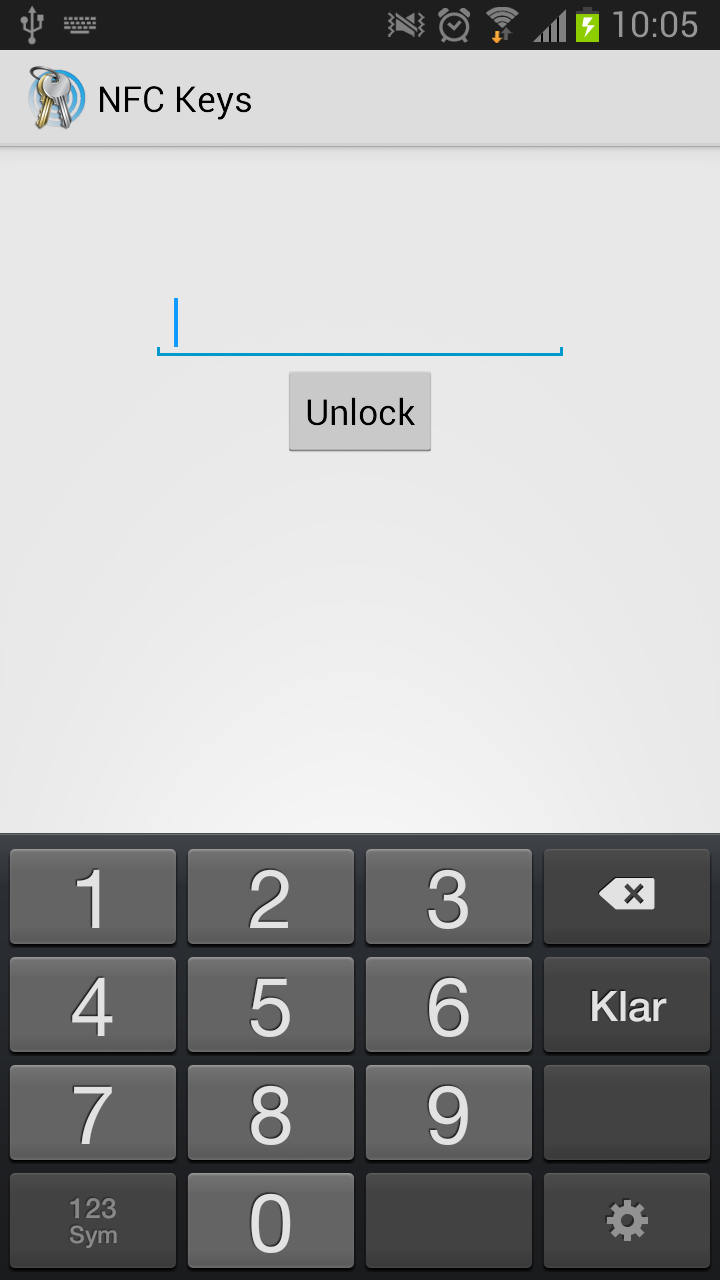
\includegraphics[scale=0.2]{app_login.png}
\caption{Login activity}
\label{fig:App_login}
\end{figure}

\subsubsection{Login}
Login är den första aktiviteten som en användare av Android-applikationen möts av, se figur x. Den huvudsakliga funktionen av denna aktivitet är att förhindra att applikationen kan användas av oönskade användare. Den fungerar som en port till övriga applikationen genom att implementera ett system för personverifiering med hjälp av PIN-kod. Ges inte rätt PIN-kod går inte övriga delar av applikationen att nå. När korrekt PIN-kod har angivits startas en timer. Timern loggar ut användaren igen efter en bestämd tid. 

% \ref:{fig:App_login}

\subsubsection{Main}
När användaren angett PIN-kod möts han av nästa aktivitet, Main. Main är aktiviten hela applikationen bygger runt. Den är ansvarig för kommunikationen och att automatiskt skicka rätt NDEF-meddelande utgående från det senaste mottagna meddelandet. Detta sker helt enligt ovanstående kommunikationsprotokoll. Användaren informeras om förloppet med hjälp av en textvy, lokaliserad nedtill. När kommunikationen har nått sitt mål, en upplåst dörr, eller om detta inte skulle ske skickas användaren vidare till Success-aktiviten alternativt Denied-aktiviteten. Är det inkommande meddelandet däremot delning av en nyckel kommer det upp en bekräftelseruta där en bekräftelse från användaren krävs innan nyckeln läggs till i databasen.

Om användaren har behov av av att ändra inställningar för applikationen trycker denne på Settings-knappen lokaliserad längst ned på skärmen för att komma till Settings-aktiviteten.

\subsubsection{Success och Denied}
Success-aktiviteten har till uppgift att visa för användaren att upplåsningen lyckades. Vid ett anrop visas aktiviteten bara en kortare stund för att sedan avslutas och applikationen går tillbaka till Main-aktiviten. Förutom Success finns det även en liknande aktivitet kallad Denied. Den har till uppgift att visa vad som gick snett om något går snett vid låsförfarandet. För övrigt fungerar den på samma sätt som Success.

\subsubsection{Settings}
Settings-aktivteten nås via knappen längst ner i Main. Aktiviten har till uppgift att rada de inställningar som finns att göra. Prototypen innehåller endast två sådanna men aktivten är förberedd för fler. Trycker användaren på knapparna kommer denne vidare till aktiviterna Password respektive Keys.

\subsubsection{Password}
Denna aktivitet har den enkla uppgiften att ändra PIN-kod. För att kunna ändra PIN-kod krävs att den gamla anges korrekt.

\subsubsection{Keys}
Slutligen finns aktiviten Keys. Huvuduppgiften för denna aktivitet, som är applikationens nästa största, är att ansvara för hanteringen av nyckelpar. Bakom aktiviten ligger en lokal relationsdatabas av SQLite-typ som är ansvarig för att lagra nyckelparen. De databasfunktioner aktiviten ger ett ovanliggande skal till är att lista alla par, redigera ett par, ta bort ett, lägga till nya, söka och att dela med andra smarta telefoner med applikationen installerad.

Längst upp på skärmen återrfinns en bläddringsbar vy med alternativknappar. Vyn listar de nyckelpar som finns i databasen och det går att välja en i taget. När en knapp är vald går det att använda knapparna för att ta bort nyckelparet från databasen eller för att dela den genom knappen nedtill. Delningsfunktionen skickar användaren vidare till en annan skärm. Förs telefonen då mot en annan smarttelefon är det möjligt att dela paret genom att röra skärmen. Nedtill finns också knappar för att skapa nya nyckelpar och för att söka bland befintliga. Popup-fönster dyker upp för dessa uppgifter.

\subsection{Låsenheten}
Den utvecklade låsenheten implementerar de nödvändiga delar utav NFCs kommunikationsstack vilka möjliggör  kommunikation via Android Beam. Vidare stödjer låsenheten säker kommunikation genom användandet av krypteringsalgoritmen RSA med 512-bitars nycklar. 

Mikrokontrollern stödjer den funktionallitet vilken krävs för att hantera kommunikation med skölden. En minimalistisk implementaion, dvs. de kommandon som utgör kärnan vid aktiv kommunikation, används. Kommunikation mellan mikrokontroller och sköld utförs med I2C som kommunikationsprotokoll. Skölden, PN532 NFC/RFID Shield, har kompletterats med en mindre diod-krets vilken indikerar om förloppet är lyckat eller ej.

Låsenheten  erbjuder ett adekvat stöd för aktiv NFC-kommunikation. Den tillhandahållna NFC-stacken består av 
minimalistiska implementationer av NDEF, SNEP och LLCP. De avkall vilka har gjorts har resulterat i begränsningar på mängden data vilket kan skickas mellan NFC-enheterna samt att endast en uppkoppling kan ske åt gången. Gränsen på data från applikationslager ligger på 250-byte per sändning. När diverse headers plockas bort resulterar detta i en datamängd på 226 byte för ren applikationsdata. Vid sändning kan en datamängd på 163 byte skickas vilket ger 139 byte för ren appliationsdata.  LTO har satts till 800ms vilket är tillräckligt även för de långsammare Android telefonerna. De mobiltelefoner vilka låsenheten har kommunicerat mot via Android Beam är HTC One X, Samsung Galaxy S3(GT-I9300) och LG Optimus L5(E 610). 

Detaljerad redogörelse av slutgiltligt arbetsförlopp för låsenhet:

\begin{itemize}
\item Vid uppstart körs Arduinos setupfunktion som tar cirka 750 ms.
\item Därefter utväxlas ett identifikationsmeddelande, vilket tar cirka 4.3 sekunder.
\item Sedan skickar mobilapplikationen ett upplåsningskommando eller ett nyckelbyteaskommando. Svar ges på detta kommando och förloppet tar cirka 4.6 sekunder.
\item Kommandot packas sedan upp, vilket tar  16ms.
\item Kommandots argument måste sedan dekryppteras vilket tar cirka 3,5 sekunder.
\item Förloppet som följer kan ske lite olika beroende på vilket kommando som skickades och dess innehåll:

\begin{itemize}
\item Om kommandot är av upplåsningstyp och den tillhörande nyckeln är korrekt läggs ingen tid på.
\item Om kommandot är av upplåsningstyp och den tillhörande nyckeln är felaktig läggs ingen tid på.
\item Om kommandot är av nyckelbytestyp och den tillhörande nyckeln är korrekt läggs 14 ms på förloppet.
\item Om kommandot är av nyckelbytestyp och den tillhörande nyckeln är felaktig kostar detta ingen extra körningstid.
\end{itemize}

\item Feedback diod vid cirka 14 sekunder.
\item Feedback till felefon ges efter 19 sekunder.
\end{itemize}

Har optimerats något... Måste göras om! yay!

Låsenheten stödjer dekryptering av 512-bitars RSA. Detta är det enskilda delmoment i mikrokontrollerns arbetsbörda vilket tar längst tid. Dekrypteringen tar cirka 3.2 sekunder av den totala körningstiden som beräknats till ca 15 sekunder på Arduino Mega 2560. 

I befintlig implementation används en standard-nyckel vid första uppstart. Användaren ges möjlighet att konfigurera denna nyckel genom välja denna funktionalitet i applikationen. Dessa nycklar lagras i mikrokorntrollerns EEPROM vilket gör att nyckeln förblir densamma, dvs. antingen den som användaren ställt in eller standardnyckeln, om låsenheten blir utan ström. 

För att sänka energiförbrukningen försätts låsenheten i ett strömsparläge då dess tjänster inte behövs. Mikrokontrollern väcks av en signal som skölden skickar när den detekterar ett NFC fält. Om även mikrokontrollern tillåts vara aktiv hela tiden fås en nominell strömförbrukning på ….. . Med strömsparfunktioner landar den på …...

För att åstadkomma dessa resultat har de flesta av kodbilbioteken till stor grad modifierast eller i extrema fall helt bytts ut. Av det som ärvts från Embedded PN532 är det endast de NDEF-relaterade som lämnast helt orört. Den kod som hanterar kommunikation mot har skölden har modifierats på så vis att  I2C används istället för SPI. Vissa kommandon som skickas ser annorlunda ut och ger skölden lite annat beteende och en strömsparfunktion har laggts till. LLCP relaterad kod har modifierats till den grad att endast vissa metodnamn kan tillskrivas Embedded PN532. Kod som haterar konstruktion av specifika ramar, mer korrekt uppkopplingshantering vilket inkluderar hantering av SAP och sekvensnummer och metoder som sköter kommunikationsförloppet mer autonomt har lagts till. Transportprotokollet NPP har ersatts med SNEP som är helt egen implementerat. All debugginformation sköts på ett mer plattseffektivt sätt, där fixa strängar placeras på Flash och allt debuggrelaterat laddas upp vilkorligt.

Summan av alla modifikationer och additioner resulterar i att mikrokontrollerns drivrutiner omfattas av 2500 rader C++ kod. Kompilerat och uppladdat på Arduinon tar detta 28880 byte av de totalt 256kbyte som finns tillgängliga. Runtime kontroller av användandet av SDRAM har uppgått till maximalt 4209 byte av 8kbyte.  

\section{Diskussion}
%Saxat från fackspråk föreläsning om retorik
%Introduktion
%Påminner läsaren om det
%övergripande problemet i
%studien, sammanhanget,
%rapportens syfte, och vilken
%typ av undersökning som
%gjorts för att komma fram till
%resultatet

Studiens syfte var att redogöra för hur ett låssystem kan designas och implementeras. I början av studien identifierades tre huvudutmaningar vilka kan sammansättas i att åstadkomma en säker kommunikation mellan en Android-enhet och en Arduiono-baserad mikrokontroller. Enheterna skall tillsammans utgöra ett låssystem. För att lyckas med detta har en omfattade studie av de relevanta teknikerna gjorts för att sedan användas i ett konstruktionsinriktat projekt.
  
%”Sammanfattning”
%= en (kort) översikt över
%studiens genomförande,
%datainsamling, analysstrategi
%och resultat (i viss mån)

Arbetet har angripits på ett iterativt sätt och har flutit på enligt förväntan när det gäller Android-applikationen. När det däremot gäller mjukvaran för mikrokontrollern har en del problem stötts på som inte hade tagits med i beräkningen.  Detta gjorde att slutprodukten inte har all den funktionalitet och inte fyller alla de krav som satts upp från början. Men resultatet är trots allt en prototyp som fungerar bra i sitt sammanhang.

%Diskussion – vad vi har kommit fram till 
%Belyser och lyfter fram det anmärkningsvärda, 
%nya, överraskande, 
%intressanta och sätter det i relation till 
%det kända inom fältet, genom:
%Konsekvens : Detta
%innebär…
%(vad betyder det ?)
%Kritisk reflektion: stämmer
%överrens? Går emot? Hur ska
%detta tolkas ?
%Påverkar resultatet och
%slutsatserna vi drar vår
%förståelse för problematiken i
%fråga? Kommer det vi har
%kommit fram till att påverka
%hur man genomför andra
%studier inom detta område?
%Hur förhåller sig det vi har
%kommit fram till teorin: tillför
%det något, går det emot eller
%bekräftar teorin?
%Påverkar vidare forskning: hur
%kan man gå vidare nu? Har det
%uppstått nya frågor som vi/man
%inte kunde förutse
%Begränsningar: kända ”brister”
%i metoden” och hur man skulle
%kunna komma runt i dem
%framtida studier

\subsection{Prototypen som helhet}
Protokollet - begränsar snabbheten, vi har haft enkelhet som fokus och ej snabbhet lite dumt när båda är varandras motsats. En lösning där endast ett meddelande hade kunnat skickats riktning hade varit enkelhet då man i förväg hade fått välja vilket lås man skulle låsa upp men en sådann hade varit snabbare. Sparat en del tid. Förloppet i sin helhet skulle då tagit en sändning och en dekryptering.

En motsvarande upplåsningsprocess utförd med två Androidtelefoner går mycket fortare. behöver kunna klocka en sändning med android på något sätt.

Krypteringen kanske hade kunnat lösas bättre. Tänk på vår diskussion kring AES och säker kanal.
Krypteringen gör oss långsamma.

En annan vanlig metod för kryptering är så kallad symmetrisk kryptering, med symmetrisk kryptering finns det enbart en privat nyckel. Denna är nyckel är hemlig och används för både kryptering och dekryptering. Det stora problemet med symmetrisk kryptering är att nyckeldistribution blir väldigt svår att hantera. Om någon angripare får tag på den hemliga nyckeln så räcker det inte med att låsenheten behöver ny nyckel dessutom behöver alla applikationer med tillgång till detta lås även få den nya nyckel distribuerad till sig. Det insågs ganska fort att detta skulle bli ett problem. Detta hade kunnat gå att lösa med en central databas som hanterar och distribuerar nya nycklar men det sågs som ett projekt som sträcktes utanför ramarna för grundidén med upprättning av kommunikation över NFC.

Hybrid-kryptosystem - borde använts istället för asymmetrisk kryptering, hade varit en elegantare lösning!
Allah rekommenderar en krypteringsmetod för NFC kommunikation beskriven i A Lightweight RFID Protocol to protect against Traceability and Cloning attacks av Tassos Dimitriou. Hade denna används istället hade beräkningskostnader kunnas hålla nere och förloppet hade snabbats upp på låsenhetssidan. 

Det påstås i teorin att 1024 bitars RSA rekommenderas men vi använder bara 512 bitar, varför?

Psuedorandom tal generaras av låsenheten vid kommunikation , kan det äventyra säkerheten? Skulle en tidsstämpel fungera bätrre än pseudorandomtal? 

Hur skyddar vi oss mot Rubber-Hose attacker?(Diskussion inget annat)

Vart försvinner tiden under förloppet?  

Olika versioner av android.

kryptering, varför valdes RSA, varför är algoritmen lämplig i vårat syfte, jämfört med AES som också undersöktes, hur hade krypteringen kunnat förbättras med bättre mikrokontroller(8-bitars vis större). Nu har vi även  till viss del disskuterat hur krypteringsbiten kan förbättras med RSA som nycketutbytning och AES som huvudkrypto efter en inledade “pairing”. Kanske hade kunnat spara massvis med tid då AES är mer Arduino-vänlig.

-Hur mycket minne krävs för krypteringen
-Är krypteringen tillräckligt säker för våran applikation

Referera till Assa Abloys NFC-låssystem

I de uppsatta kraven finnns
d begränsar?(Kanske antennen är seg )

\subsection{Mobilapplikationen}
Svårigheter
Vana java-programmerare löste de mesta problemen som uppstod, med hjälp av developer.android.com och hemsidan Stack Overflow som visdomskälla.\\
-Ett problem som uppstod var att variabler inte sparades när aktiviteter stängdes. Ta upp lite om detta
Shared Prefs osv. Bug i keypair gjorde detta ytterliggare svårare. Bouncy castle\\
-Något som hade varit önskvärt hade varit ett sätt att “overridea” Android-Beam-rutan som tar hela skärmen. Det hade gjort appen tydligare mer lättförstålig(enhetlig).\\
-Central enhet med distrubitionsansvar för nycklar hade varit bättre.men jobbigare

\subsection{Låsenheten}
Fint generellt intro till hela låsenheten...
Detta har visat sig genom krånglande programvara och oförklarliga kompileringsfel som enligt principen många bäckar små sinkat utvecklingsprocessen.

\subsubsection{Arduino}
Efter att ha arbetat med Arduino har det insetts att Arduino-plattformen inte är en färdigutvecklad plattform. Detta är inte förvånande då plattformen inriktar sig mot utveckling av hobbyprojekt. Vidare har upphovsmännen bakom plattformen gjort den till öppen källkod för att uppmuntra användarna att sjävla utveckla plattformen. Tyvärr sammordnar inte upphovsmännen denna utveckling nämnvärt och den har därmed skett mer eller mindre sporadiskt. Detta har resulterat i att dokumentationen av ett källkodsbibliotek är generellt undermålig. Ett konkret exempel på detta är Arduinos implementation av I2C-kommunikation där bristande information kring bufferstorlekar ledde till obegripliga fel. 

Utvecklingsmiljön Arduino tillhandahåller är minst sagt simpel. Den ger ingen möjlighet till att ge insyn i hur kod kompileras och inte heller några verktyg med vilka kompilering kan styras. Ett problem, vilket fick oss att inse behovet av insyn och kontroll vid kompileringen, uppstod när projektet växt sig stort och komplicerat. Kompilatorn valde då en hoppinstruktion vilken inte täckte hela addressrymden som projektet tog i anspråk. Detta fick som följd att koden inte alls fungerade och mycket tid gick åt till att hitta felkällan. Stöd för debugging finns i form av utskrifter via konsol och mer utvecklade verktyg skulle behövts då alla buggar inte kan hittas via utskrifter, till exempel pekarfel vilka kan vara svåra att upptäcka. Är man inte föriktig kan den uppladdade koden förstöras och exkivering och följaktligen utskrifterna upphör. Detta sätt att debugga är allså mycket ineffektivt och debuggingprocessen tar längre tid än den skulle gjort om bättre verktyg fanns. Dessutom plågas utvecklingsmiljön av en del buggar varav den mest påstridiga är att kontakten med mikrokontrollern tappas gång efter annan. Allt detta har lett till att det totala intrycket av IDE:n inte är till dess förtjänst.

Vi har i efterhand hittat utvecklingsmiljön Atmel Studio, vilken är betydligt mer komplicerad än den utvecklingsmiljö Arduino erbjuder. Atmel Studio erbjuder mer utvecklad debugging och både insyn och kontroll av kompileringen. Vi gjorde ett försök att få till stånd en övergång men det visade sig vara alltför komplicerat att från Atmel studio få tillgång till den Arduinospecifka kod som projektet baserats på. Om vi från början vetat om detta alternativ så hade vi försökt använda det från början.

\subsubsection{Implementering}
Trenden med odokumenterad kod drabbade tyvärr de källkodsbilbiotek vilka vi valde att basera vår impmementation på. Istället för att kunna läsa i en överskådlig dokumentation har vi istället fått lusläsa i koden, vilket är en process som tagit mycket av vår tid.

Problemen vilket tagit överlägset mest tid är dem vilka relaterar till implementationen av NFC-stacken. Det har visat sig mycket svårt att från specifikation av stackens relevata delar gå till en fungerande implementation. Specifkationerna lämnar en del att önska, framförallt vad gäller tolkningsvänlighet. Hade det inte varit för det andra SNEP-projekt (Lotito 2013) vilken implementerade förloppen på ett fungerande sätt, så hade vi antagligen forfarande haft problem med kommunikationen.

Tolkningsproblem verkar också vara förekommande bland mobiltillverkarna vars implementationer av NFC-stacken tycks skilja sig åt sinsemellan. NFC-implementaionen på HTC one X skiljer sig åt från Samsung galaxy S3. Detta tycks inte bero på hårdvarumässiga skillnader som kan härledas till NFC-chippet. Båda telefonerna använder samma chip från NXP semiconductors. Att hårdvara spelar in har vi bekräftat med hjälp av LG-telefonen. Den ter sig vara för långsam för att kunna hantera NFC-kommunikation i de hastigheter vi kräver. Alla skillnader som förekommer kan antagligen härledas till att NFC är en relativt ung teknik. Alla standarder och tillhörande implementationer har till synes inte rotat sig lika djupt som de har gjort hos äldre tekniker. Om några år när NFC har uppnått en högre grad av mognad och standarder och implementationer satt sig, tror vi att NFC kan bli något rikgitg stort. 

En del avkall har gjorts för implementationen av NFC-stacken i detta projekt. Detta medför att, om vi ämnat att släppa låssystemet för komersiellt bruk, inte kan få låsenheten NFC-certifierad. De delar utav NFC-stacken vilka inte implementerats är de delar vilka vi inte ansåg vara nödvändiga för att utveckla en låsenhet med den sökta funktionalliteten (se 4.1 Produktkrav). Avkallen gjordes också för att vi bedömde det orimligt att implementera hela NFC-stacken på den tid vi hade till förfogande. för att minska storleken på koden och minnesanvändningen. Att på ett inbyggt system, i alla fall de baserat på arduinoplattformen, få plats med en fullständing NFC implementation bedömde vi som orimligt, framförallt då arbetet var tidsbegränsat. 

På NDEF-lagret så stödjer vi enbart sändandet av Short-records och enbart ett enskillt record. Vidare är inte chunking-mekanisken implementerad. Förklaringen till detta är att vårt låssystem enbart skickar meddelnaden som maximalt är 256-byte långa och enbart består av ASCII formaterad text. Således fanns det inget behov att implementera stöd för mer flexibel hantering av NDEF-meddelanden. 

SNEP protokollet är implementerat så att funktioanalitet inom projektets ramar kan utföras. Eftersom data ska skickas mellan enheterna och detta kan utföras genom att endast skicka PUT-förfrågningar och implementation GET-förfrågningar kräver yttligare komplexitet, så gjorde valet att implementera endast stöd PUT-förfrågningar. Inte heller har feedback, i form av SNEP-meddelanden, till sändaren implementeras då ett fel uppkommer eller någon form av felrättande kod. Istället gjorde valet att då ett fel uppkommer så startar upplåsningsförloppet om.

På LLC nivå är det länkanteraren som inte till fullo har den funktionalitet som specificeras av NFC-forum. Vår implementation en uppkoppling nästintill korrekt. För att ha en helt korrekt hantering av en uppkoppling skall LLC hålla reda på dels det lokala mottagningsfönstret (3.1.1.3) men även det hos mottagar LLC. I aktuell implementation görs ingendera. Vidare så har inte LLC möjlighet att hantera flera aktiva sessioner vilket också specificeras av NFC-forum. Korrekt hantering av mottagningsfönster hade relativ enkelt kunnat implementeras, men eftersom dessa inte utgjorde någon begränsning under sändförloppet hade dessa inte fyllt någon funktionalitet. Att implementera stöd för flera parallella uppkopplingar bedömde vi som alltför komplext och tidskrävande för att rymmas inom projektets ramar. Dessutom ställer vi oss tveksamma till om det alls hade varit möjligt att implementera på en Arduinoplattform som begränsad beräkning och minneskapacitet.

Lite snabba tankar kring de Svårigheter vi stött på:

C: C programmering är besvärlig. Man är nere på nästan lägsta nivån och måste hålla koll på pekare etc. Vidare ardunio har sina egenheter.

Ardunio: Arduino må vara välanvänt, men inte alltför väldokumenterat. Dolda buffertstorlekar, vad som faktsikt läggs var på minnet och diverse andra egenheter som t.ex. serial out print som muppar till sig ibland. Svårtolkade fel som ibland kan härledas till minnesbrist och i andra fall finns det ingen rimlig förklaring.

LLC: Förvisso väldokumenterat men inte lättare att förstå för det. Antingen tolkar vi det fel, eller så är det något som inte riktigt stämmer. Vi ska t.ex. inte behöva skicka symm-frames som vi gör då enheterna turas om om att skicka data till varandra?

Arduinos utvecklingsmiljö är mongo och skapar buggar som egentligen inte finns. 

Kryptering: Beräkna nycklar och dekryptering är tunga beräkningar och optimeringar behövde utföras. källkodsbibliotek som användes behövde vara optimerade för begränsad beräkningskapacitet som mikrokontrollern hade att tillgå.


\section{Slutsats}
Hur gick projektet? 
Nådde vi våra mål?
Hur är vår syn på effektmålen, kan de förverkligas?

\textcite{article:Allah}
\textcite{online:Android_popular}

\newpage
\section*{Referenslista}

\printbibliography[]

\newpage
\section*{Bilagor}

\subsection*{Kravspecifikation}
Skallkrav är de krav som måste uppfyllas av vår konstruktion medan börkrav är de krav som ses som sekundära. Börkraven är fördelaktiga att uppfylla och leder till en mer fullständig produkt.
Skallkrav för produkten som helhet
\begin{enumerate}
\item Endast användare med de rätta uppgifterna ska kunna agera mot  låset.
\item Kommunikation mellan mobilapplikation och låsenheten sker via NFC.
\item Kommunikationen mellan enheterna skall vara krypterad
\item Låset skall kunna låsas upp/låsas inom fem sekunder.
\end{enumerate}
Börkrav för produkten som helhet
\begin{enumerate}
\item Upplåsningsprocessen/låsningsprocessen bör vara snabb nog för att låset skall vara upplåst låst inom 1 sekund efter att kommandot skickats.
\item Låsenheten bör kunna konfigureras av mobilapplikation.
\item Det bör vara möjligt för flera användare att operera mot samma lås alternativt begränsa antalet telefoner som har tillåtelse att låsa upp låset.
\end{enumerate}
Specifika Börkrav för mobilapplikation
\begin{enumerate}
\item Vid förbättring av designen bör utvecklingen följa Jacob Nielsen’s heuristik[3].
\item Noga testad och har inga kända buggar.
\item Mobilapplikationen bör fungera på samtliga Androidtelefoner utrustade med NFC.
\item Nycklar bör kunna delas mellan olika Androidtelefoner över en NFC-länk.
\item Implementera personverifiering med PIN-kod i mobilapplikation.
\end{enumerate}
Specifika Börkrav för låsenhet
\begin{enumerate}
\item Felsäker, t.ex. vid strömavbrott bör låset förbli låst.
\item Formfaktorn bör vara anpassad för ändamålet.
\item Lösningen bör inte dra för mycket ström vid normal användning.
\end{enumerate}

\subsection*{Kravverifiering}
Verifiering av skallkrav:
\begin{enumerate}
\item hejj
\item Låsenhetens funktionalitet kan enkelt testas genom att låta den skriva ut ett meddelande till terminalen när den tagit emot data. För att testa om peer-to-peer kommunikation har uppnåtts kan låsenheten efter att ha mottagit data skicka ett svar till telefonen. Telefonen skriver i sin tur ut svaret på skärmen.
\item För att undersöka om meddelanden som skickas är krypterade tillåts låta en tredje enhet lyssna på en konversation mellan telefon och låscontroller. Om meddelandet inte är i klartext eller är alltför enkelt att tyda bedöms krypteringsmålet som uppfyllt.
\item Personverifiering testas i mjukvaran genom att se om programmet beter sig rätt då en korrekt PIN-kod ges.
\item Tidskravet som ställts för upplåsning verifieras genom att starta en timer i mobilapplikationen då upplåsningskommandot/låsningskommandot skickas och sedan stoppa timern då ett svar mottagits från låsenheten.
\end{enumerate}

Verifiering av börkrav för produkten som helhet:
\begin{enumerate}
\item Se verifiering av skallkrav punkt 4.
\item När konfigureringsfunktionen är implementerad testas den genom att låta mobilapplikationen skicka önskad konfigureringsinformation till låsenheten. Sedan genomförs en vanlig upplåsning under vilken applikationen och kontrollerns beteende jämförs mot det beteendet som beskrivs i konfigureringen.
\item Om flera mobiltelefoner tillåts skicka kommandon mot låsenheten en i taget är kravet verifierat om avsedd funktion utförs. Alternativet, att enbart en telefon tillåts låsa upp låset, verifieras genom att använda en annan otillåten telefon och undersöka om låset förblir låst.
\end{enumerate}

Verifiering av specifika börkrav för mobilapplikation:
\begin{enumerate}
\item Utvärdering om att Jacob Nielsens heuristik har följts.
\item För att eliminera buggar kommer applikationen genomgå rigorös testning under vilken i de mer framträdande buggarna rättas.
\item Om mobilapplikationen körs och fungerar korrekt på flera olika telefoner tillverkade av olika företag och/eller som kör olika
androidversioner anses detta mål uppnått.
\end{enumerate}
Verifiering av specifika börkrav för låsenheten:
\begin{enumerate}
\item Genom att återskapa de situationer som produkten är ämnad att klara av kan låset observeras för att kontrollera att det trots situationen agerar korrekt.
\item Om låsenheten kan implementeras i praktiken, det vill säga inte vara större än ett vanligt låshus till en vanlig dörr, har detta krav uppnåtts.
\item När låsenheten kan styra en elektrisk låskolv så är det här kravet uppfyllt.
\end{enumerate}

\newpage
\subsection*{Rapport om individuella bidrag}
Detta stycke ska vara med. Ine allt för omfattande så vi skjuter på denna tills det drar ihop sig. Rapporten slerp3D i pingpong ger ett exempel.
Ansvarsområden
\begin{itemize}
\item Planering
\item Informationsinhämtning/inläsningsdel
\item Metoder -- val/utveckling
\item Genomförande
\end{itemize}
Bidrag till problemlösning, syntes och analys
\begin{itemize}
\item Problemlösning 
\item Kreativitet, idérikedom
\item Skapande av modell
\item Analys av projektrelaterat material 
\item Diskussionsbidrag
\item Slutsatser
\end{itemize}
Huvudansvarig författare av avsnitt
\begin{itemize}
\item Avsnitten anges
\item Eventuell redaktionell ansvarsfördelning bör anges
\end{itemize}


\end{document}
